\section{Objetivos}
\begin{frame}%[shrink=10]
  \frametitle{Objetivos del día}
  \begin{itemize}
  \item Entender que es un cluster computacional y como funciona.
  \item Procedimiento para Conseguir una Cuenta en Apolo y Responsabilidades.
  \item Ingreso a Apolo desde y fuera de la Universidad.
  \item Compilación en gcc y gfortran
  \item Sistema de Colas: Como lanzar trabajos en Apolo
  \item Paseo!
  \end{itemize}
\end{frame}

\section{¿Qué es un Clúster Computacional?)}

\begin{frame}
  \texttt{``Supercomputación, también llamada Computación de Alto Rendimiento ha sido reconocido por el Congreso (Norteamericano) como vital para la prosperidad de la nación, seguridad nacional y económica, producción industrial, ingeniería y avances científicos.''}
  \begin{flushright}
    \small{Tomado de: About Supercomputing -- NASA Ames Research Center.}
  \end{flushright}
\end{frame}

\begin{frame}
  \frametitle{Paradigmas de la Ciencia}
  \begin{itemize}
  \item Miles de años atrás la ciencia era empírica.
  \item Últimos cientos de años usamos modelos y generalizaciones.
  \item Últimas decadas usamos computadoras para simular fenómenos complejos.
  \item Ahora exploramos datos unificando los tres paradigmas anteriores. 
  \end{itemize}
\end{frame}

\begin{frame}
\frametitle{La Necesidad de Cómputo en Paralelo}
\begin{itemize}
\item Multinúcleo no es suficiente
	\begin{itemize}
	\item Más Memoria
	\item Más Procesamiento
	\item Más Almacenamiento
	\end{itemize}
\item Simulación
	\begin{itemize}
	\item Astronomía: Astrofísica, Exobiología...
	\item Ingeniería: Física, Civil, Mecánica, Aerodinámica...
	\item Seguridad: Física, Informática, Criptografía, Forense...
	\item Medicina: Farmacéutica, Bioinformática...
	\end{itemize}
\end{itemize}
\end{frame}

\begin{frame}
\frametitle{Preguntas Fundamentales}
\begin{itemize}
\item ¿Qué se va a ejecutar en Paralelo?
\item ¿Se puede ejecutar en Paralelo?
\item ¿Debe existir comunicación entre procesos?
\item ¿Debe existir comunicación entre máquinas?
\begin{itemize}
	\item Monotarea (Multics, DOS)
	\item Multitarea (Unix, Linux, Windows)
	\item Distribuidos (Unix, Linux, Windows)
\end{itemize}
\end{itemize}
\end{frame}

\begin{frame}
 \begin{figure}[ht]
        \centering
        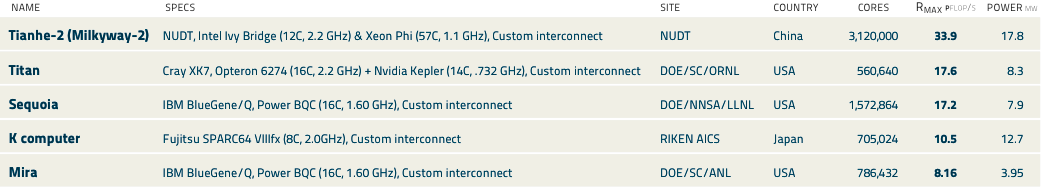
\includegraphics[scale=0.29]{imgs/top500june}
        \caption{Top 500 June}
      \end{figure}
\end{frame}

\begin{frame}
 \begin{figure}[ht]
        \centering
        \includegraphics[scale=0.2]{imgs/pleiades}
        \caption{NASA Pleiades -- \small{Tomado de Wikimedia}}
      \end{figure}
\end{frame}

\begin{frame}
 \begin{figure}[ht]
        \centering
        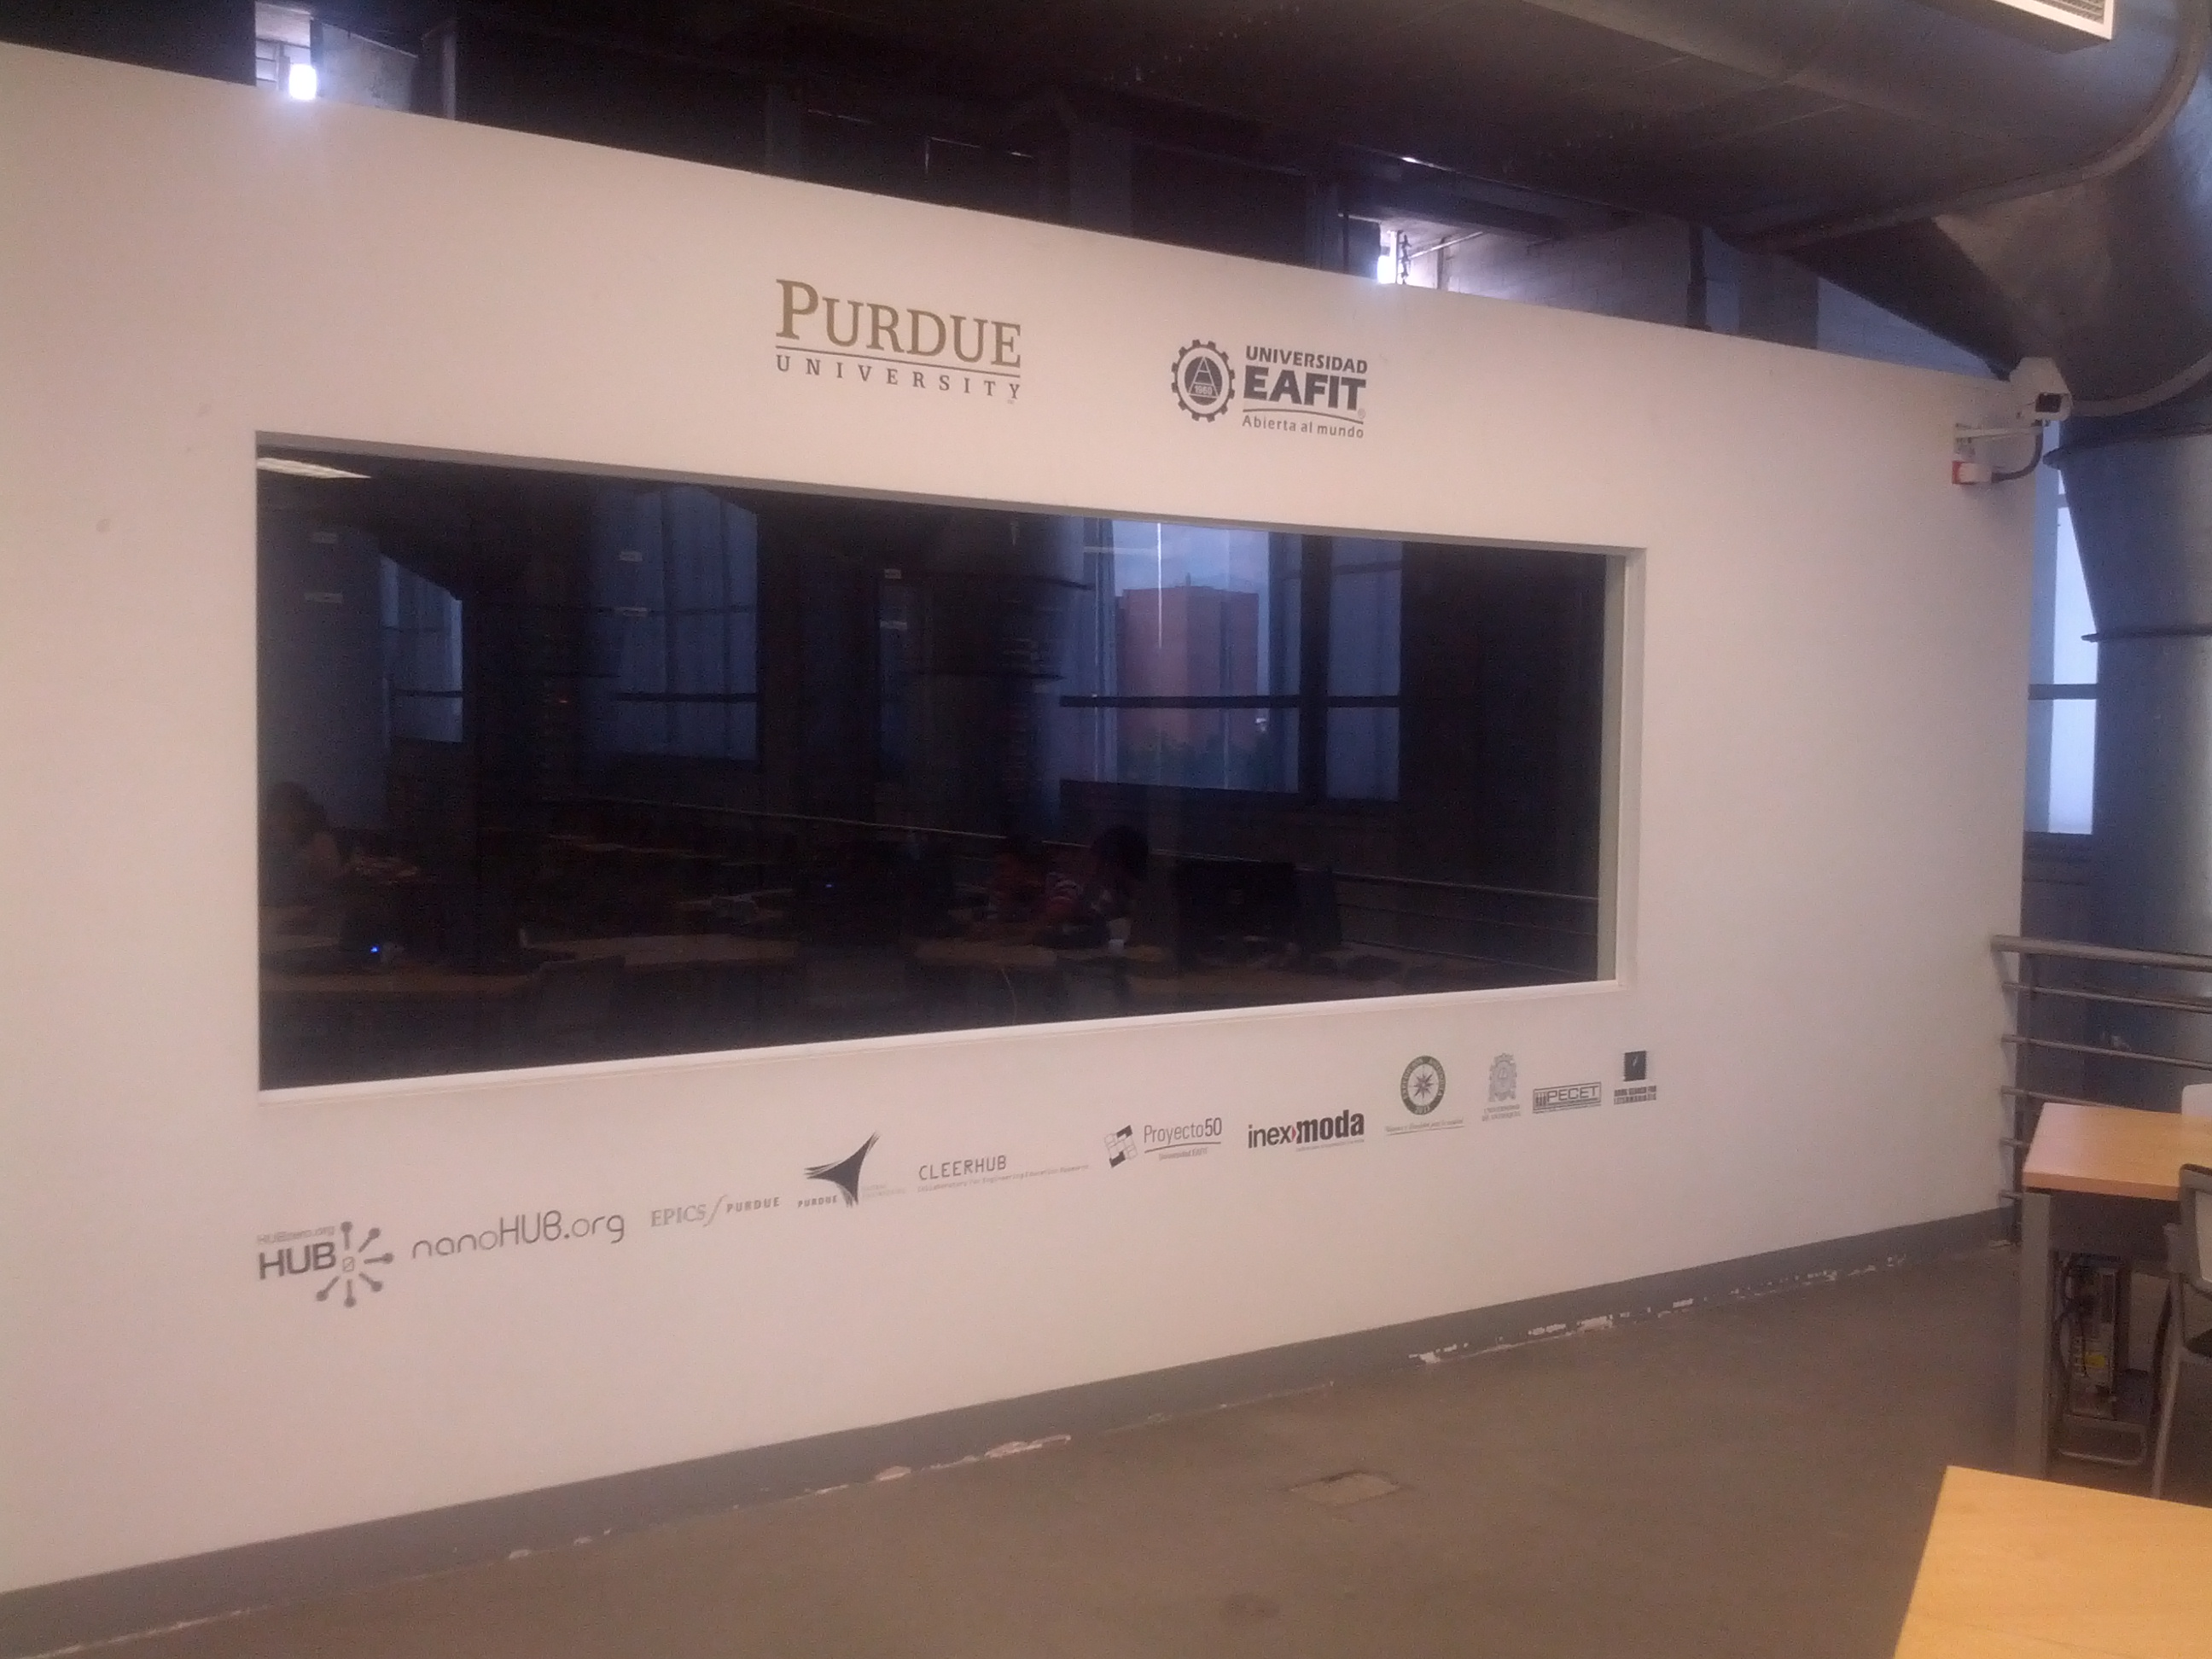
\includegraphics[scale=0.1]{imgs/apolo}
        \caption{Universidad EAFIT -- Apolo}
 \end{figure}
\end{frame}

\begin{frame}
 \begin{figure}[ht]
        \centering
        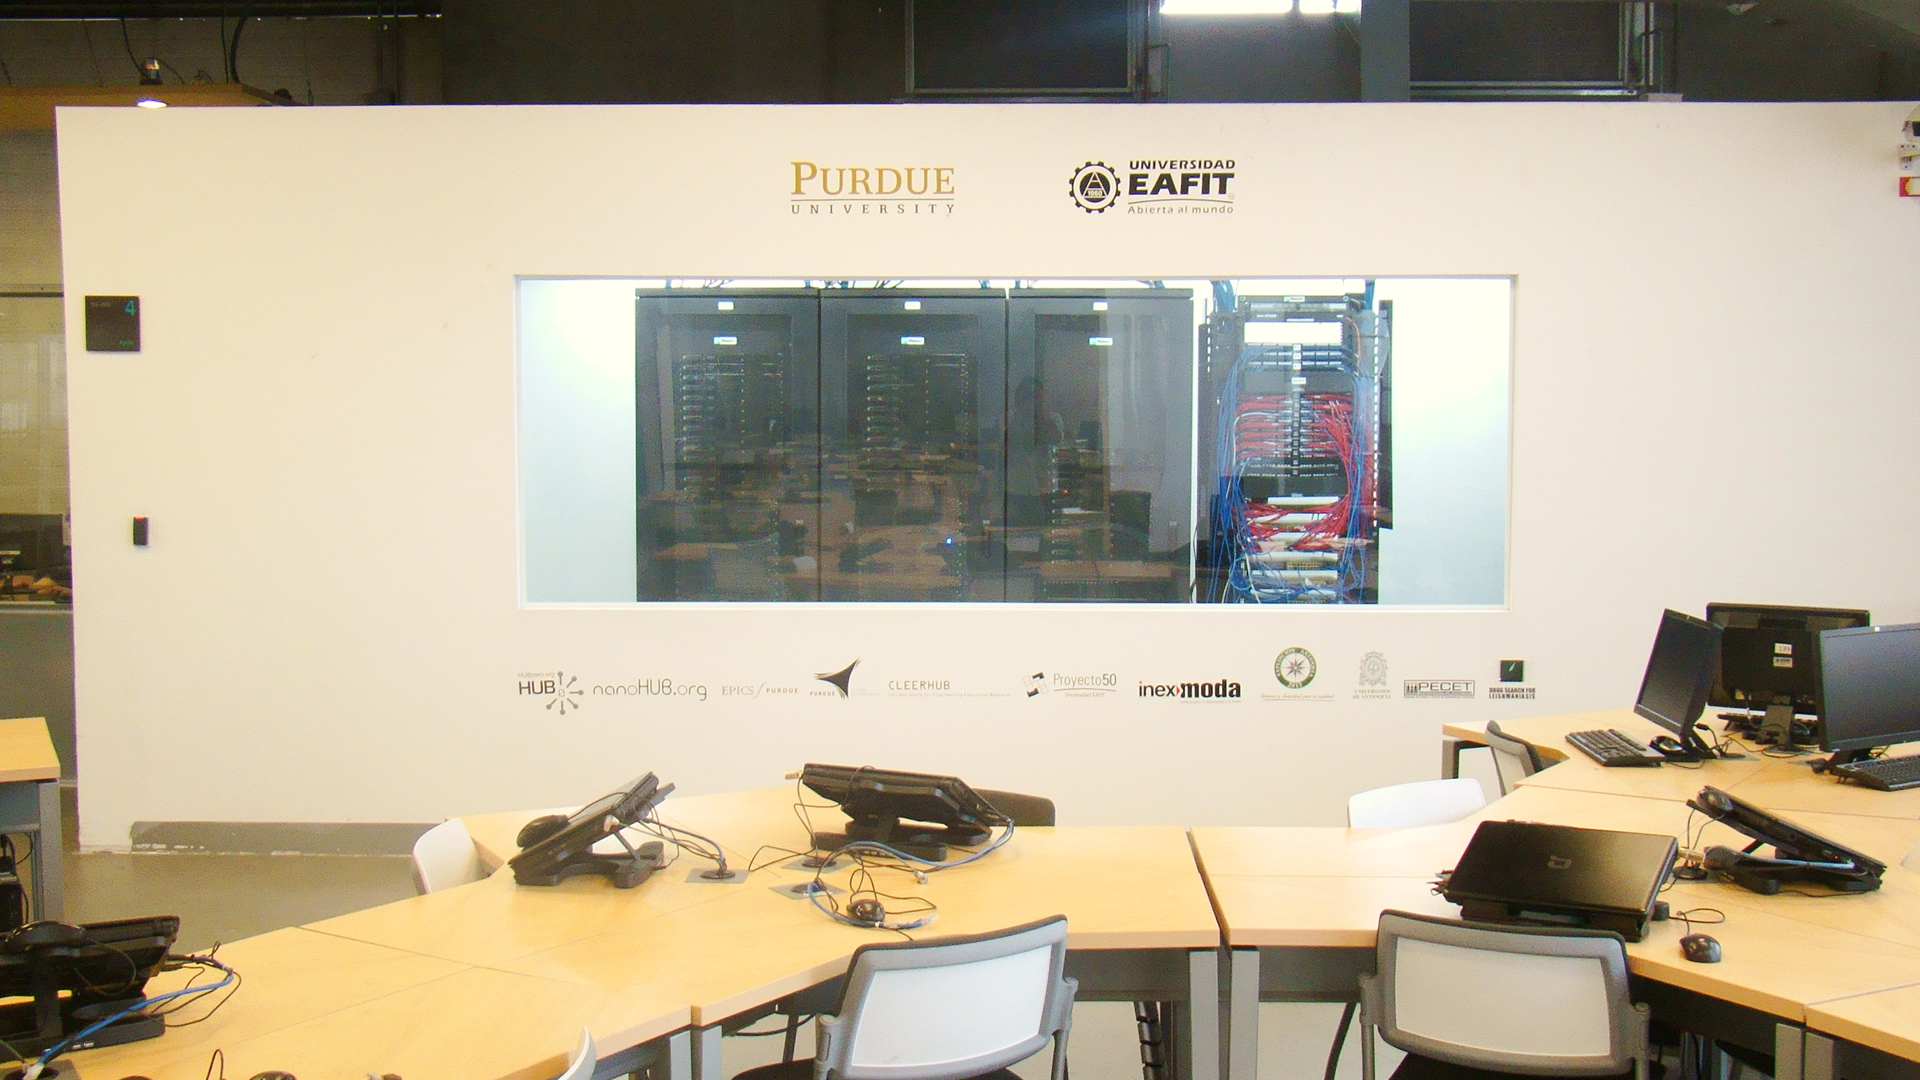
\includegraphics[scale=0.15]{imgs/apolo1}
        \caption{Universidad EAFIT -- Apolo}
 \end{figure}
\end{frame}

\begin{frame}
 \begin{figure}[ht]
        \centering
        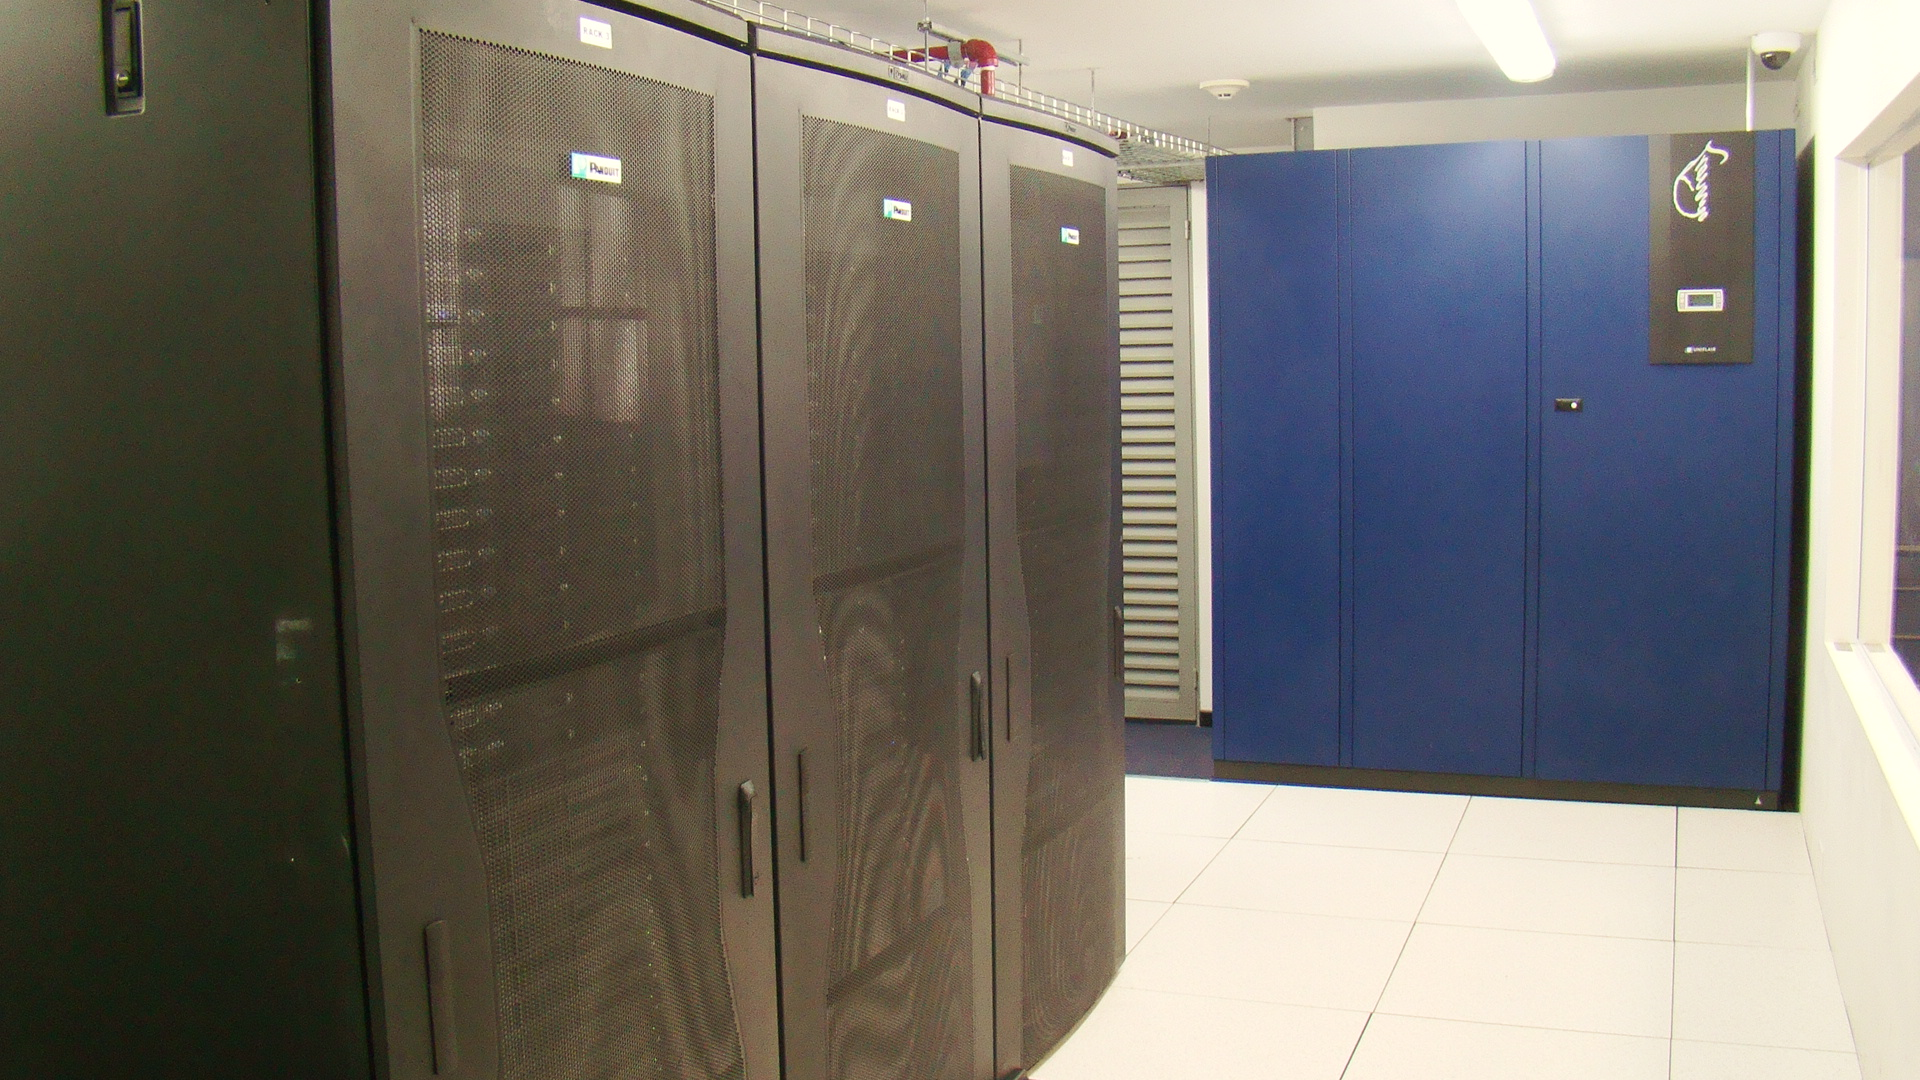
\includegraphics[scale=0.15]{imgs/apolo2}
        \caption{Universidad EAFIT -- Apolo}
 \end{figure}
\end{frame}


\begin{frame}
 \begin{figure}[ht]
        \centering
        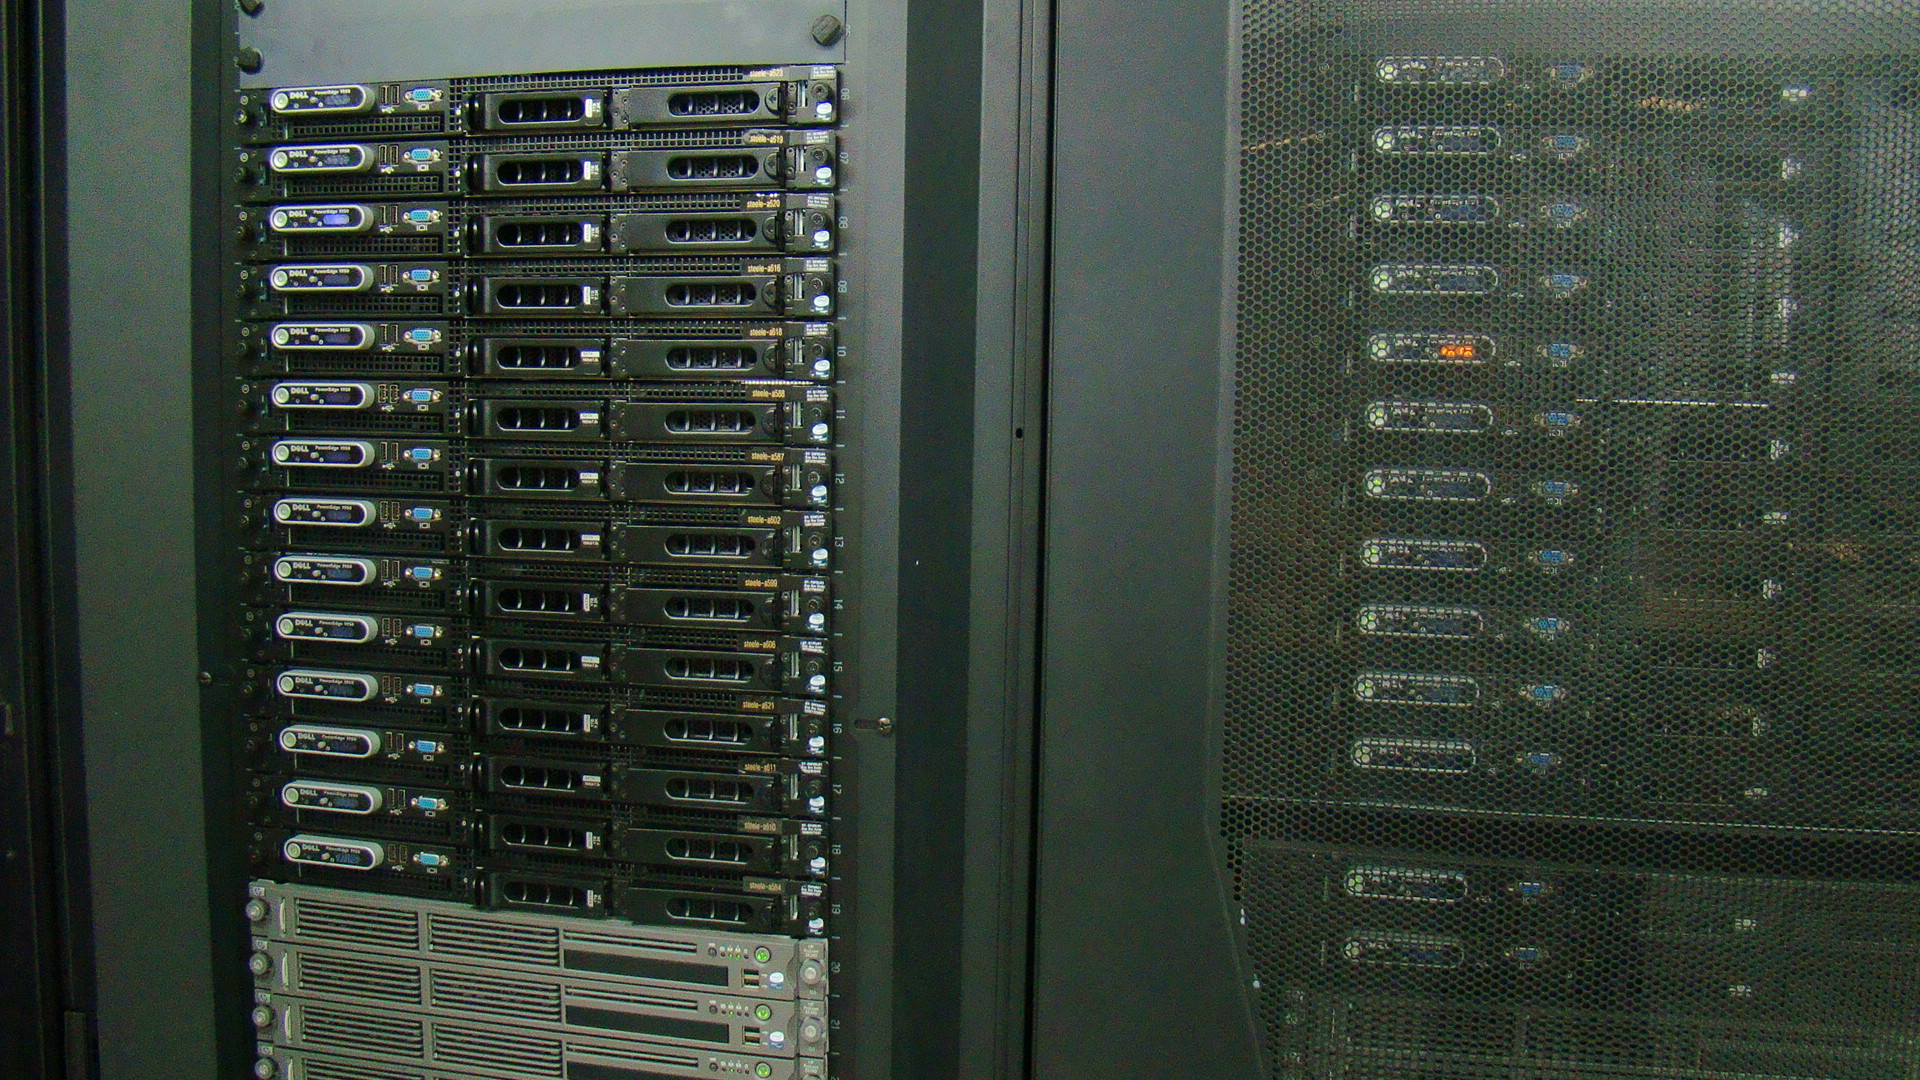
\includegraphics[scale=0.15]{imgs/apolo3}
        \caption{Universidad EAFIT -- Apolo}
 \end{figure}
\end{frame}


\begin{frame}
 \begin{figure}[ht]
        \centering
        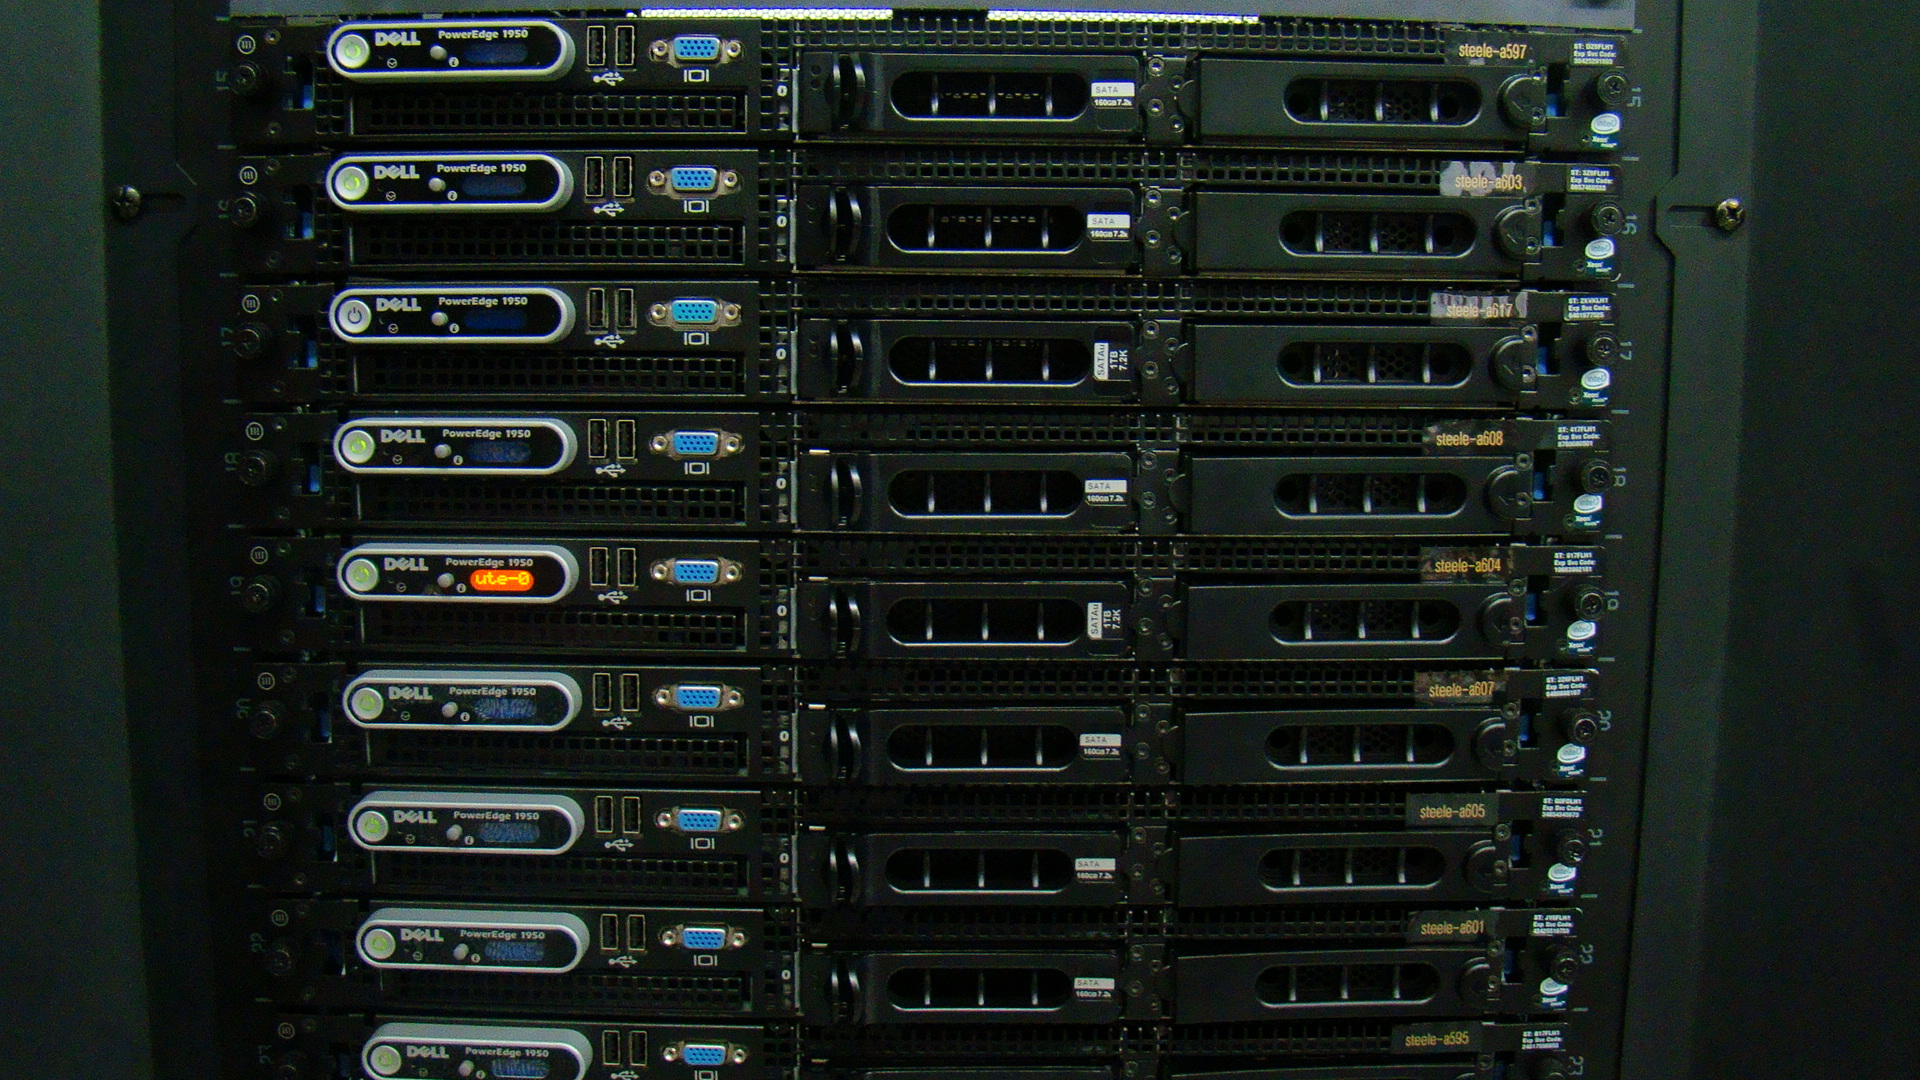
\includegraphics[scale=0.15]{imgs/apolo4}
        \caption{Universidad EAFIT -- Apolo}
 \end{figure}
\end{frame}


\begin{frame}
 \begin{figure}[ht]
        \centering
        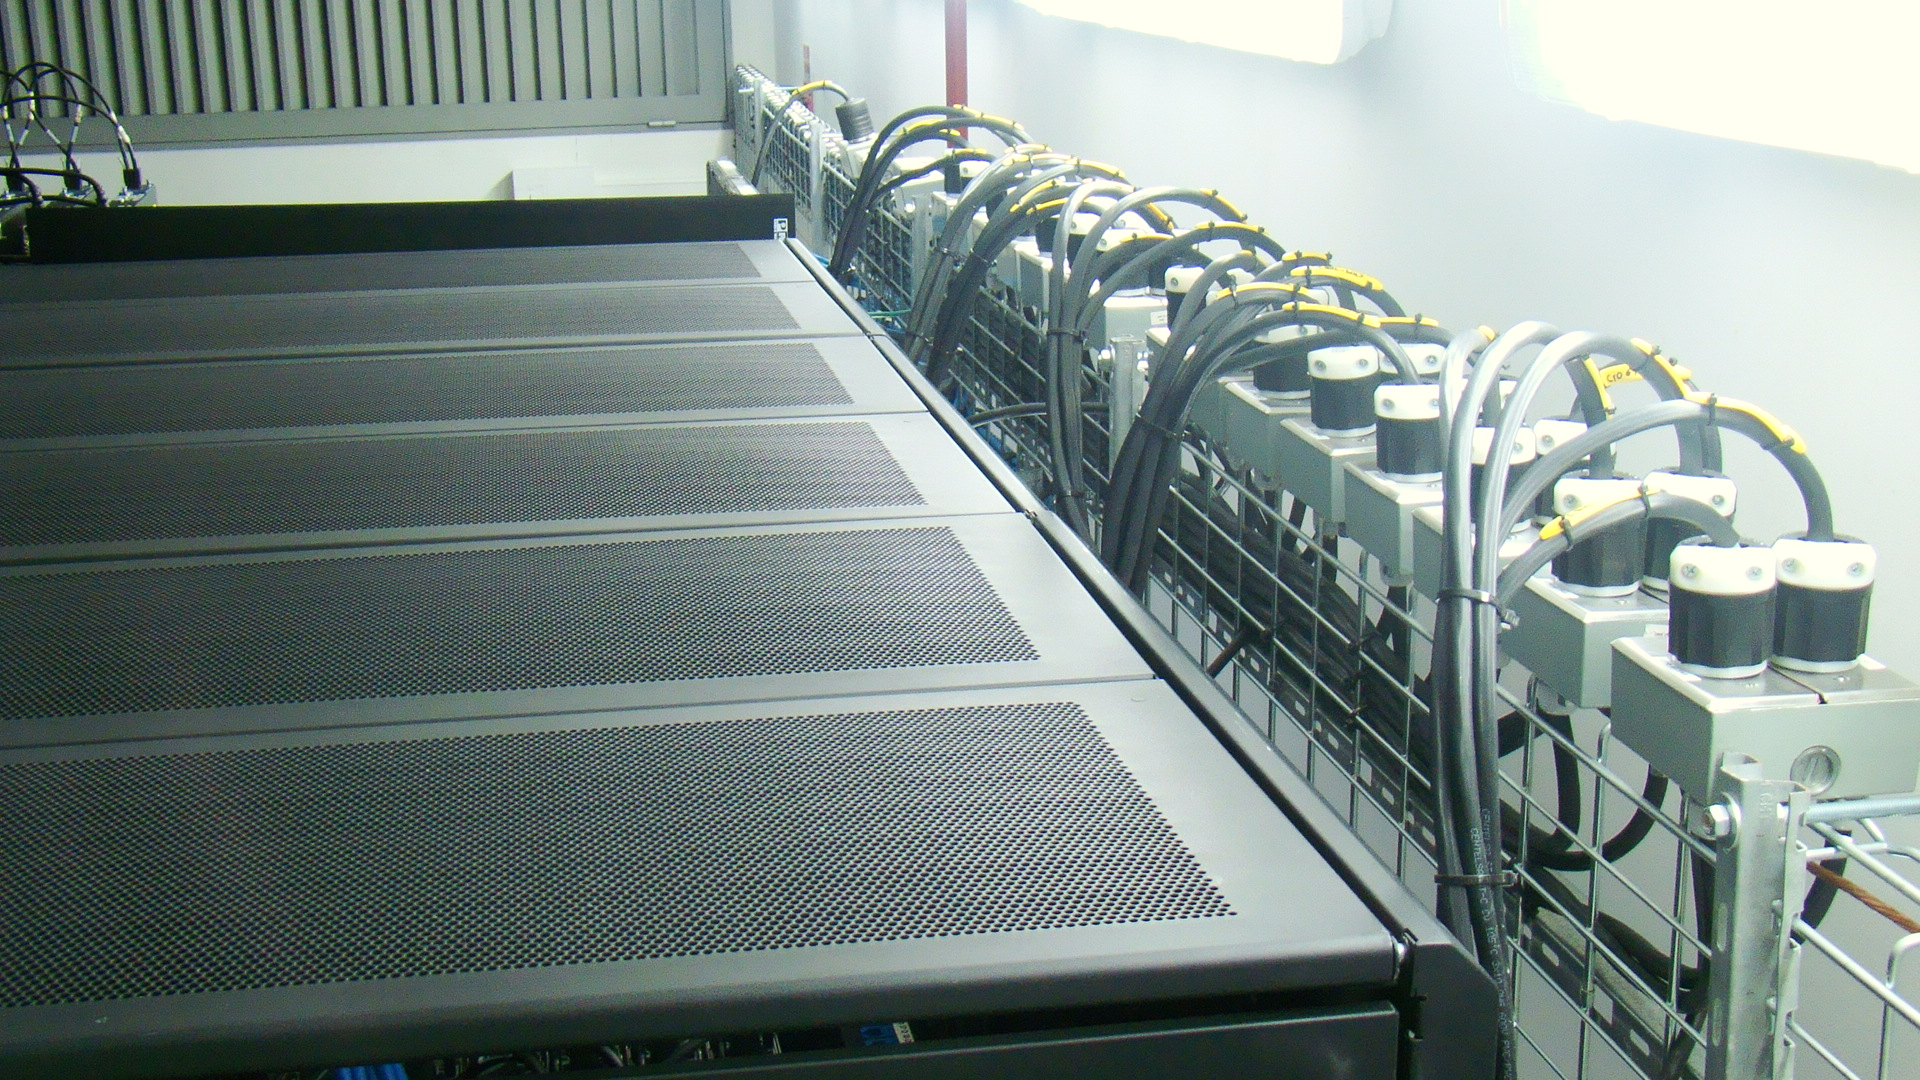
\includegraphics[scale=0.1, angle=90]{imgs/apolo5}
        \caption{Universidad EAFIT -- Apolo}
 \end{figure}
\end{frame}

\begin{frame}
 \begin{figure}[ht]
        \centering
        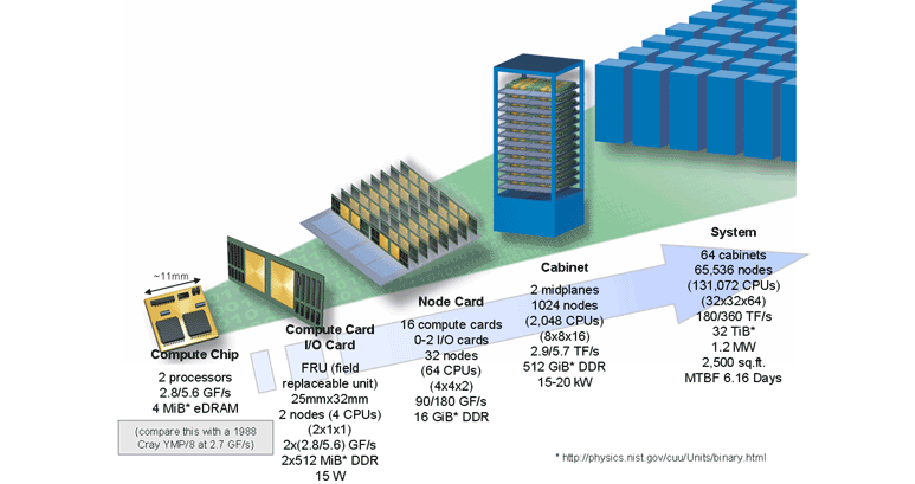
\includegraphics[scale=0.35]{imgs/bluegenearch}
        \caption{Arquitectura de un Cluster -- Blue Gene}
 \end{figure}
\end{frame}

\begin{frame}
\frametitle{Especificaciones de Apolo}
  \begin{columns}
    \begin{column}[ht]{5cm}
      \begin{itemize}
      \item 86 Máquinas
      \item 528 Núcleos
      \item Arquitectura Intel
      \item Híbrido
      \item Linux Rocks
      \item 4.7 TeraFLOPS (Teórico)
      \end{itemize}
    \end{column}
    \begin{column}[ht]{5cm}
      \begin{figure}[ht]
        \centering
        
\includegraphics[scale=0.35]{imgs/tux}
      \end{figure}
    \end{column}
  \end{columns}
\end{frame}

\begin{frame}
\frametitle{Como Conseguir una Cuenta}
  \begin{columns}
    \begin{column}[ht]{5cm}
      \begin{itemize}
      \item jpineda2@eafit.edu.co
      \item Tener cuenta activa en la Universidad
      \item Llenar formulario
      \item Configurar VPN para acceso remoto o externo a la Universidad
      \end{itemize}
    \end{column}
    \begin{column}[ht]{5cm}
      \begin{figure}[ht]
        \centering
        
\includegraphics[scale=0.35]{imgs/bobe}
      \end{figure}
    \end{column}
  \end{columns}
\end{frame}

\begin{frame}
\frametitle{Como conectarse a Apolo: VPN y SSH}
      \begin{figure}[ht]
        \centering
        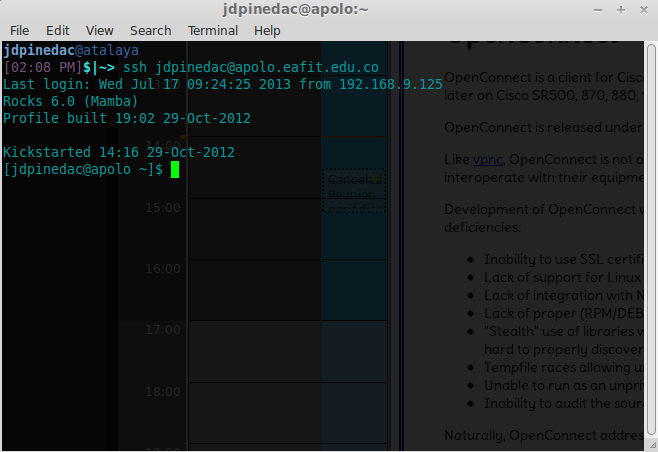
\includegraphics[scale=0.35]{imgs/ssh}
      \end{figure}
\end{frame}

\begin{frame}
\frametitle{Como compilar en C/C++}
      \begin{figure}[ht]
        \centering
        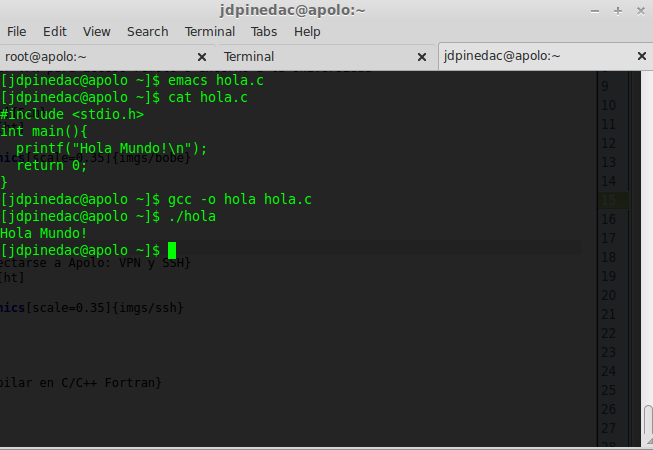
\includegraphics[scale=0.4]{imgs/gcc}
      \end{figure}
\end{frame}

\begin{frame}
\frametitle{Como compilar en Fortran}
      \begin{figure}[ht]
        \centering
        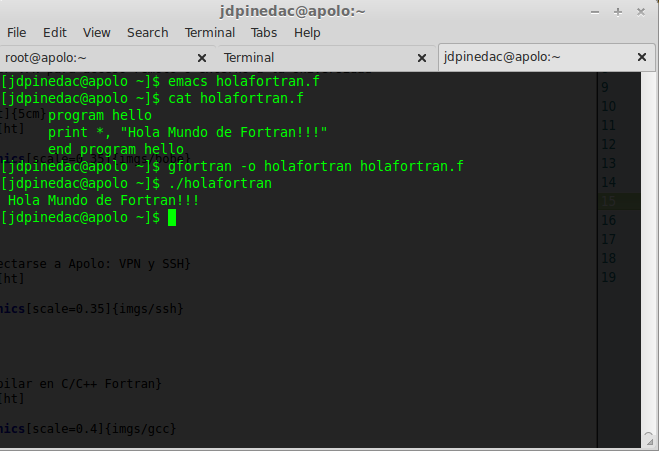
\includegraphics[scale=0.4]{imgs/fortran}
      \end{figure}
\end{frame}

\begin{frame}
\frametitle{Como Lanzar Procesos al Sistema de colas}
      \begin{figure}[ht]
        \centering
%        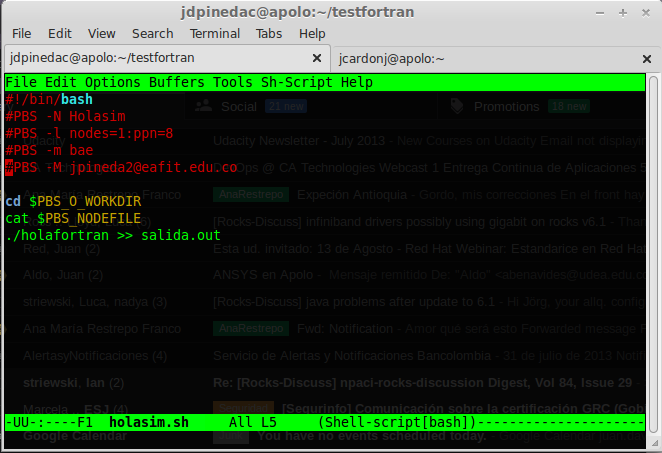
\includegraphics[scale=0.4]{imgs/queue}
      \end{figure}
\end{frame}

\begin{frame}
\frametitle{Como Lanzar Procesos al Sistema de colas}
      \begin{figure}[ht]
        \centering
        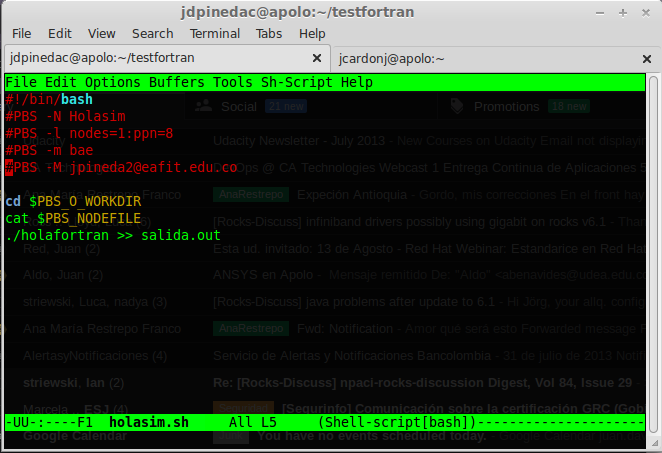
\includegraphics[scale=0.4]{imgs/queue}
      \end{figure}
\end{frame}

\begin{frame}
\frametitle{Como Lanzar Procesos al Sistema de colas}
      \begin{figure}[ht]
        \centering
        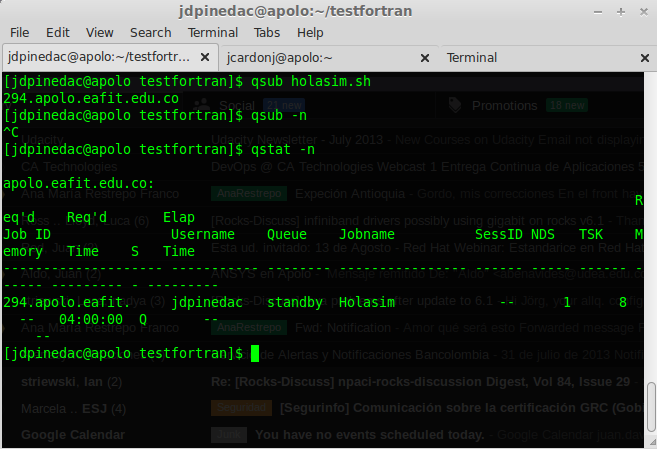
\includegraphics[scale=0.4]{imgs/queue1}
      \end{figure}
\end{frame}

\begin{frame}
\frametitle{Lecturas Recomendadas}
	\begin{itemize}
	\item HPC Traingn at LLNL -- http://goo.gl/MRBkXF
	\item Programación en Clusters Rocks -- http://goo.gl/zt71mh
	\item Stanford's Fortran 77 Tutorial -- http://goo.gl/jkYP1c
	\end{itemize}
\end{frame}

\begin{frame}
\frametitle{Paseo!}
      \begin{figure}[ht]
        \centering
        
\includegraphics[scale=0.4]{imgs/gaz}
      \end{figure}
\end{frame}




%\begin{frame}
%  \frametitle{Ken Thompson y Dennis Ritchie}
%  \begin{columns}
%    \begin{column}[ht]{5cm}
%      \begin{itemize}
%      \item Crearon Multics, luego UNIX en 1969.
%      \item Thompson diseño B, el predecesor de C.
%      \item Ambos crearon el lenguaje C en 1972.
%      \item Ganaron el premio Turing en 1983 y la Medalla Nacional de Tecnología en 1999.
%      \end{itemize}
%    \end{column}
%    \begin{column}[ht]{5cm}
%      \begin{figure}[ht]
%        \centering
%        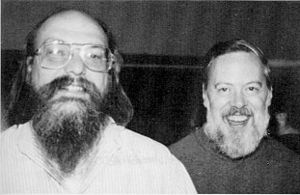
\includegraphics[scale=0.35]{imgs/ken_dennis.jpg}
%        \caption{Thompson y Ritchie.}
%      \end{figure}
%    \end{column}
%  \end{columns}
%\end{frame}
%
%\begin{frame}[shrink=25]
%  \frametitle{Vinton Cerf y Robert Kahn}
%  \begin{columns}
%    \begin{column}[ht]{6cm}
%      \begin{itemize}
%      \item Cerf: Graduado de Matemáticas y Ciencias de la Computación en Stanford, MsC y PhD en UCLA.
%      \item Kahn: MsC. y PhD. de la Universidad de Princeton.
%      \item En los 70's desarrollaron el conjunto de protocolos y el diseño de ARPANET.
%      \item Desarrollaron TCP/IP en 1972 como investigación en la Universidad de California y Stanford.
%      \item Recibieron el premio Turing en el 2004.
%      \item Recibieron el premio Príncipe de Asturias con Lawrence Roberts y Tim Berners--Lee en 2002.
%      \end{itemize}
%    \end{column}
%    \begin{column}[ht]{4cm}
%      \begin{figure}[ht]
%        \centering
%        \includegraphics[scale=0.25]{imgs/cerfandkahn.jpg}
%        \caption{Dr. Vinton Cerf y Dr. R. Kahn.}
%      \end{figure}
%    \end{column}
%  \end{columns}
%\end{frame}
%
%\begin{frame}
%  \frametitle{ARPANET}
%  \begin{itemize}
%  \item Primera red de conmutación de paquetes.
%  \item Creada por encargo del DoD a la Agencia de Proyectos de Investigación Avanzada (ARPA) luego conocida como DARPA.
%  \item Antecesora de Internet hasta 1983 que fué completamente migrada al conjunto de protocolos TCP/IP.
%  \end{itemize}
%\end{frame}
%
%\begin{frame}
%  \frametitle{Línea del Tiempo de Internet}
%  \begin{figure}[ht]
%    \centering
%    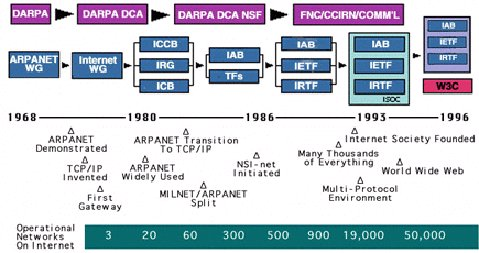
\includegraphics[scale=0.5]{imgs/timelinearpanet.jpg}
%    \caption{Linea del Tiempo ARPANET}
%  \end{figure}
%\end{frame}
%
%
%\begin{frame}[squeeze]%[shrink=10]
%  \frametitle{Tim Berners--Lee: WWW}
%  \begin{columns}
%    \begin{column}[ht]{5cm}
%      \begin{itemize}
%      \item Físico de la Universidad de Oxford.
%      \item Creador de la WWW: HTTP, HTML, URL.
%      \item Trabajó en el CERN durante la investigación.
%      \item Actualmente trabaja en la Web Semántica.
%      \end{itemize}
%    \end{column}
%    \begin{column}[ht]{5cm}
%      \begin{figure}[ht]
%        \centering
%        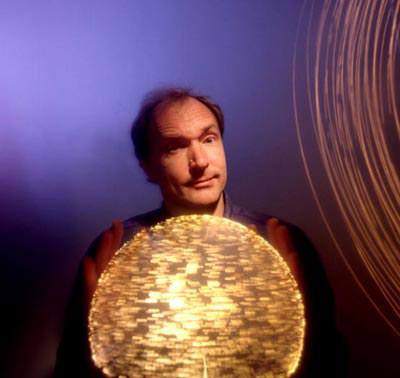
\includegraphics[scale=0.25]{imgs/tim.jpg}
%        \caption{Sir Tim Berners-Lee.}
%      \end{figure}
%    \end{column}
%  \end{columns}
%\end{frame}
%
%\begin{frame}
%  \begin{center}
%    \Huge{\textbf{¿Qué es un Hacker?}}
%  \end{center}
%\end{frame}
%
%\begin{frame}[fragile]
%  \frametitle{Eric S.Raymond}
%  \begin{columns}
%    \begin{column}[ht]{5cm}
%      \begin{figure}[ht]
%        \centering
%        \includegraphics<2->[scale=0.2]{imgs/ericsraymond.jpg}
%        \uncover<3->{ \caption{Eric Steven Raymond -- Responsable del Jargon File.} }
%      \end{figure}
%    \end{column}
%    \begin{column}[ht]{5cm}
%      \uncover<1->{``Es una persona que disfruta explorar los detalles de los sistemas programables y en el cómo aumentar sus capacidades en oposición a la mayoría de los usuarios, quienes prefieren aprender el mínimo necesario. Es una persona que le gusta tener un entendimiento íntimo de la forma como funciona internamente un sistema, computador ó red de computadores en particular''.}
%    \end{column}
%  \end{columns}
%\end{frame}
%
%%El hacker mítico Richard Stallman tiene su propia definición de hacker.
%\begin{frame}[fragile]
%  \frametitle{Richard Stallman}
%  \begin{columns}
%    \begin{column}[ht]{4cm}
%      \begin{figure}[ht]
%        \centering
%        \includegraphics<2->[scale=0.5]{imgs/richardstallman.jpg}
%        \uncover<3->{\caption{Richard Stallman -- Fundador FSF.}}
%      \end{figure}
%    \end{column}
%    \begin{column}[ht]{6cm}
%      \uncover<1->{``\textit{Hacker}, usando la palabra inglesa, quiere decir divertirse con el ingenio (\textit{cleverness}), usar la inteligencia para hacer algo difícil. No implica trabajar solo ni con otros necesariamente. Es posible en cualquier proyecto. No implica tampoco hacerlo con computadoras. Es posible ser un \textit{hacker} de las bicicletas. Por ejemplo, una fiesta sorpresa tiene el espíritu del \textit{hack}, usa el ingenio para sorprender al homenajeado, no para molestarle.''}
%    \end{column}
%  \end{columns}
%\end{frame}
%
%\begin{frame}
%  \frametitle{Definición de Hacker} %sacado de pekka himmanen, la etica del hacker.
%  \begin{itemize}
%  \item ``Programar de forma entusiasta.'' R.M.S.
%  \item ``Poner en común la información constituye un extraordinario bien.'' R.M.S.
%  \item Todo comenzó en el MIT en la década de los 60's.
%  \item En los 80's se comenzó a degenerar el término gracias a medios de comunicación.
%  \end{itemize}
%\end{frame}
%
%\begin{frame}
%  \frametitle{Ciberfauna}
%  \begin{columns}
%    \begin{column}[ht]{5cm}
%      \begin{itemize}
%      \item Cyberpunk
%      \item Über--Hacker
%      \item Hacker
%      \item Cracker
%      \item Phreaker
%      \item Lamer
%      \item Carder
%      \item Newbie o Wannabe
%      \end{itemize}
%    \end{column}
%
%    \begin{column}[ht]{5cm}
%      \begin{itemize}
%      \item Spammer
%      \item Bucanero -- Sneaker
%      \item Warez
%      \item Virri
%      \item Hacktivistas
%      \item Script--Kiddie
%      \item Nerd
%      \item Geek
%      \end{itemize}
%    \end{column}
%  \end{columns}
%\end{frame}
%
%\begin{frame}
%  \frametitle{Motivación de un Hacker}
%  \begin{itemize}
%  \item Adicción a los computadores
%  \item Curiosidad de lo que es posible
%  \item Entusiasmo
%  \item Status Social
%  \item Poder
%  \item Mejoramiento de la sociedad
%  \end{itemize}
%\end{frame}
%
%\begin{frame}
%  \frametitle{Diferencia entre Hacker y Cracker}
%  \begin{center}
%    \huge{\textbf{\alert{AUTORIZACIÓN}}}
%  \end{center}
%\end{frame}
%
%\begin{frame}[shrink=5]
%  \frametitle{The White Hats.}
%  \begin{columns}
%    \begin{column}[ht]{5cm}
%      \begin{figure}[ht]
%        \centering
%        
\includegraphics[scale=0.1]{imgs/tux.png}
%        % \caption{Tux.}
%      \end{figure}
%      \begin{itemize}
%      \item Richard Stallman -- Free Software Foundation.
%      \item Steve Wozniak -- Construyó un computador porque no tenía dinero suficiente.
%      \item Linus Torvalds -- Creador de Linux.
%      \end{itemize}
%    \end{column}
%    \begin{column}[ht]{5cm}
%      \begin{figure}[ht]
%        \centering
%        \includegraphics[scale=0.25]{imgs/gnu.png}
%        % \caption{GNU.}
%      \end{figure}
%      \begin{figure}[ht]
%        \centering
%        \includegraphics[scale=0.25]{imgs/apple.jpg}
%        % \caption{Apple.}
%      \end{figure}
%    \end{column}
%  \end{columns}
%\end{frame}
%
%\begin{frame}[shrink=10]
%  \frametitle{La Catedral y el Bazar -- Eric S. Raymond}
%  \begin{enumerate}
%  \item Todo buen trabajo de software comienza a partir de las necesidades personales del programador.
%  \item Los buenos programadores saben qué escribir. Los mejores, qué reescribir (y reutilizar).
%  \item ``Contemple desecharlo; de todos modos tendrá que hacerlo.'' (Fred Brooks, The Mythical Man-Month, Capítulo 11)
%  \item Si tienes la actitud adecuada, encontrarás problemas interesantes.
%  \item Cuando se pierde el interés en un programa, el último deber es heredarlo a un sucesor competente.  
%  \end{enumerate}
%
%  Referencia: http://biblioweb.sindominio.net/telematica/catedral.html
%\end{frame}
%
%\begin{frame}[fragile]
%  \frametitle{En esos días...}
%  \begin{flushright}
%    \textit{``... sucedió que había un joven estudioso en Helsinki, de nombre Linus el Torvalds. Linus era hombre devoto, un discípulo de RMS y seguidor acérrimo del espíritu de Turing, Von Neumann y Moore. Un día cayó en trance y tuvo una visión...''}
%  \end{flushright}
%  \begin{flushleft}
%    \small{Evangelio según Tux.}
%  \end{flushleft}
%\end{frame}
%
%\begin{frame}
%  \frametitle{Ley de Linus}
%  \begin{center}
%    \large{\textbf{``Dado un número suficientemente elevado de ojos, todos los errores se convierten en obvios''.}}
%  \end{center}
%\end{frame}
%
%\begin{frame}
%  \frametitle{¿Qué es GNU/Linux?}
%  \begin{columns}
%    \begin{column}[ht]{5cm}
%      \begin{itemize}
%      \item Sistema Operativo Multiusuario, Multitarea, similar a Unix.
%      \item Bajo Licencia GPL.
%      \item Creado por un finlandés, en 1991.
%      \item Linux es el Kernel.
%      \item Nace como respuesta a \textit{Minix}.
%      \end{itemize}
%    \end{column}
%    \begin{column}[ht]{5cm}
%      \begin{figure}[ht]
%        \centering
%        
\includegraphics[scale=0.03]{imgs/tux2.png}
%        %\caption{}
%      \end{figure}
%    \end{column}
%  \end{columns}
%\end{frame}
%
%\begin{frame}
%  \frametitle{Linus Torvalds -- Creador de Linux}
%  \begin{columns}
%    \begin{column}[ht]{5cm}
%      \begin{figure}[ht]
%        \centering
%        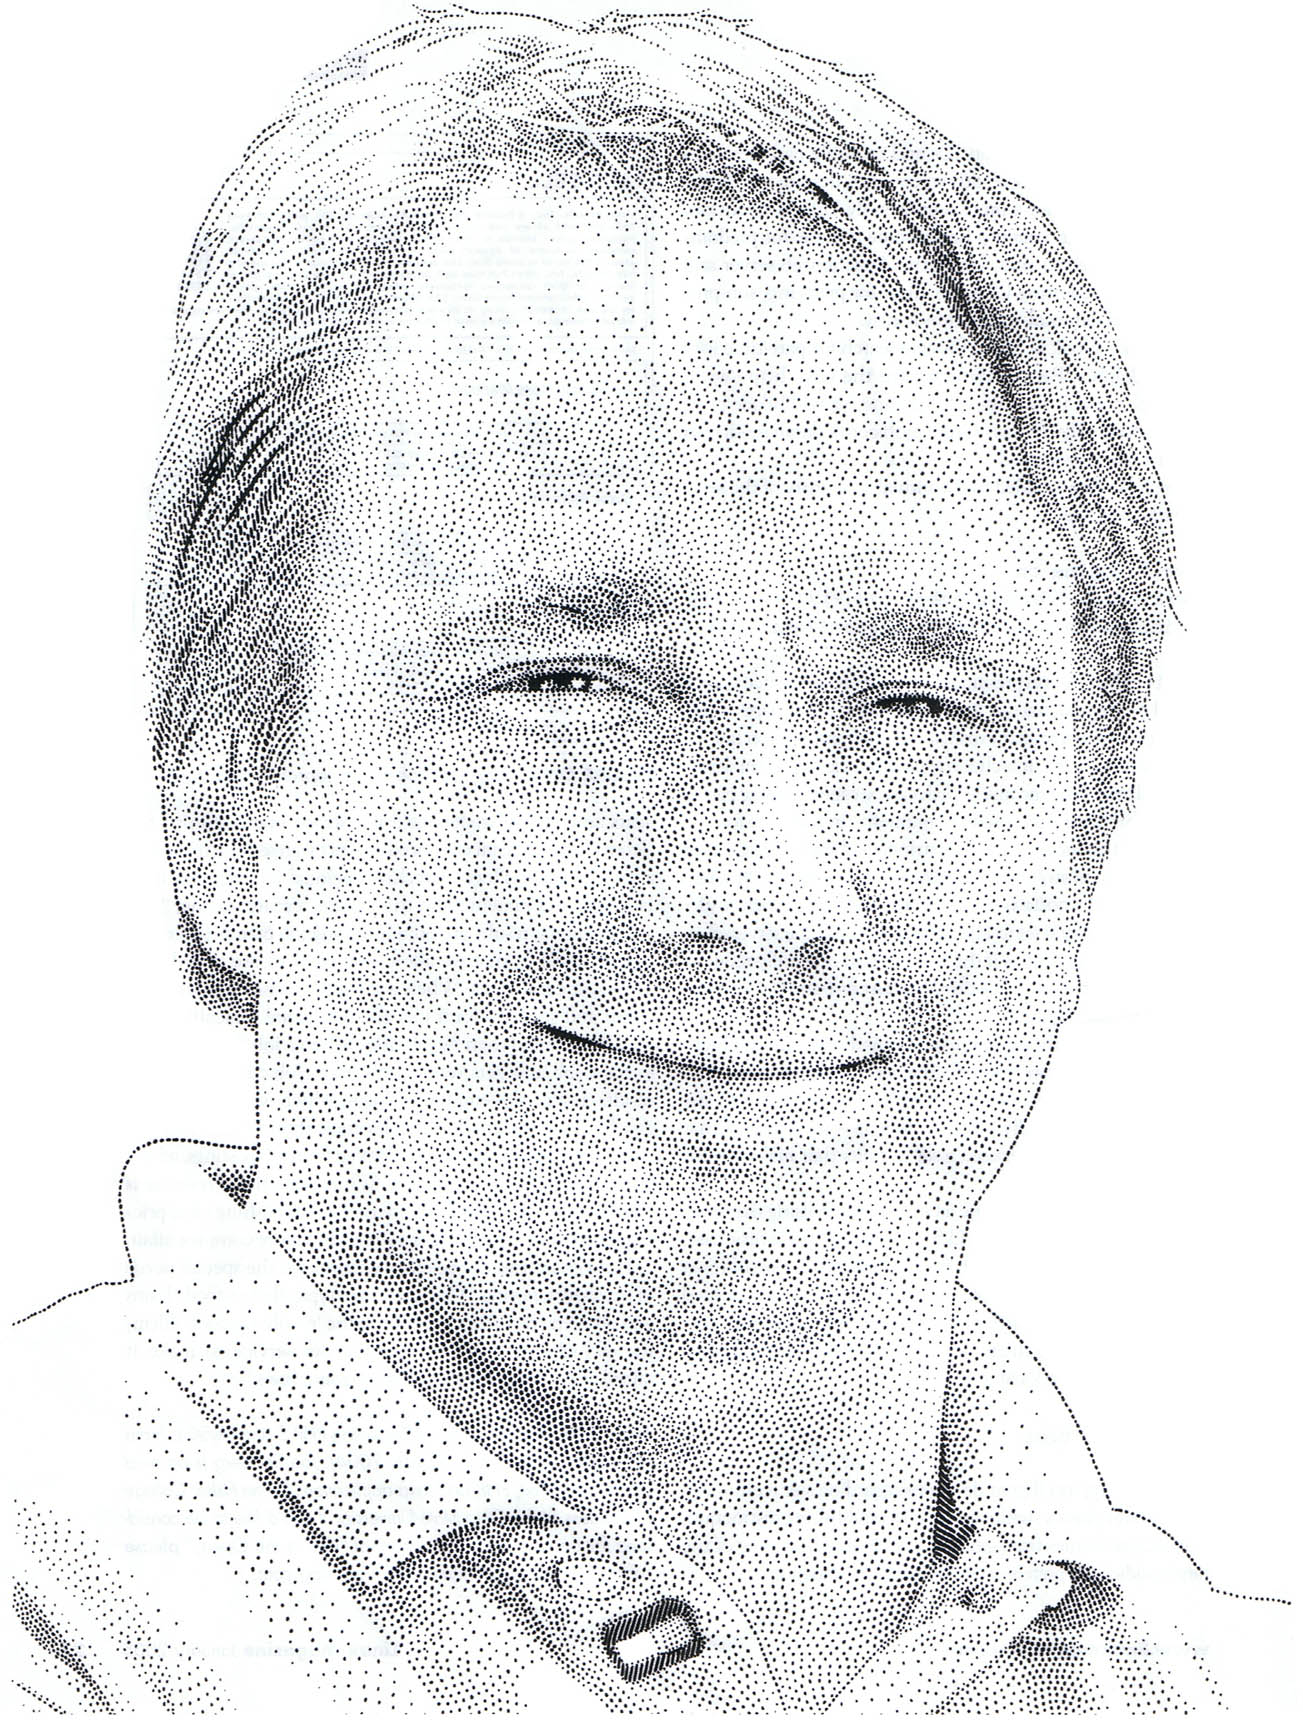
\includegraphics[scale=0.25]{imgs/linusdots.jpg}
%      \end{figure}
%    \end{column}
%    \begin{column}[ht]{5cm}
%      \begin{figure}[ht]
%        \centering
%        \includegraphics[scale=0.35]{imgs/linusteam.jpg}
%      \end{figure}
%    \end{column}
%  \end{columns}
%\end{frame}
%
%\begin{frame}
%  \frametitle{Software Libre}
%  \begin{columns}
%    \begin{column}[ht]{5cm}
%      \begin{itemize}
%      \item También conocido como Open Source.
%      \item Respeta la libertad de los usuarios sobre un producto adquirido.
%        \begin{itemize}
%        \item Ejecutar
%        \item Copiar
%        \item Distribuir
%        \item Estudiar
%        \item Cambiar
%        \item Mejorar
%        \end{itemize}
%      \end{itemize}
%    \end{column}
%    \begin{column}[ht]{5cm}
%      \begin{figure}[ht]
%        \centering
%        \includegraphics[scale=0.35]{imgs/gnutux.jpg}
%        \caption{GNU y Tux.}
%      \end{figure}
%    \end{column}
%  \end{columns}
%\end{frame}
%
%\begin{frame}
%  \frametitle{Software Libre}
%  \begin{figure}[ht]
%    \centering
%    \includegraphics[scale=0.33]{imgs/mapconcept.png}
%    \caption{Mapa Conceptual del S.L.}
%  \end{figure}
%\end{frame}
%
%\begin{frame}
%  \frametitle{Software Libre: Libertades}
%  \begin{itemize}
%  \item \textbf{Libertad 0:} Usar el programa con cualquier propósito.
%  \item \textbf{Libertad 1:} Estudiar cómo funciona el programa y modificarlo adaptándolo a tus necesidades.
%  \item \textbf{Libertad 2:} Distribuir copias del programa, con lo cual puedes ayudar a tu prójimo. 
%  \item \textbf{Libertad 3:} Mejorar el programa y hacer públicas esas mejoras a los demás, de modo que toda la \underline{comunidad} se beneficie.
%  \end{itemize}
%\end{frame}
%
%\begin{frame}
%  \frametitle{Linux Prodigio}
%  \begin{figure}[ht]
%    \centering
%    \includegraphics[scale=0.5]{imgs/comunidad.png}
%    \caption{IBM Ad.}
%  \end{figure}
%  \centering{http://www.youtube.com/watch?v=F5WLEu4UIds}
%\end{frame}
%
%
%\begin{frame}[shrink=10]
%  \frametitle{Software Libre: Licencias}
%  \centering{Algunas de las más conocidas son:}
%  \begin{columns}
%    \begin{column}[ht]{5cm}
%      \begin{itemize}
%      \item GPL
%      \item LGPL
%      \item Apache
%      \item PHP
%      \item Mozilla
%      \item MIT
%      \item BSD
%      \item Creative Commons
%      \end{itemize}
%    \end{column}
%    \begin{column}[ht]{5cm}
%      \begin{figure}[ht]
%        \centering
%        
\includegraphics[scale=0.25]{imgs/apache.jpg}
%      \end{figure}
%      \begin{figure}[ht]
%        \centering
%        
\includegraphics[scale=0.25]{imgs/cc.jpg}
%      \end{figure}
%      \begin{figure}[ht]
%        \centering
%        
\includegraphics[scale=0.15]{imgs/gpl.png}
%      \end{figure}
%    \end{column}
%  \end{columns}
%  \centering{Puede encontrar las licencias reconocidas en: http://www.opensource.org/licenses/alphabetical}
%\end{frame}
%
%\begin{frame}[fragile]
%  \frametitle{}
%  \begin{centering}
%    \centering{\textit{``Hijos de Von Neumann, oídme. IBM y las corporaciones de las CPUS encadenaron a vuestros antepasados con graves y peligrosas licencias, hasta tales extremos que clamabais a los espíritus de Turing y Von Neumann implorando vuestra liberación. Ahora yo os digo: soy más poderoso que cualquiera de las corporaciones que me precedieron. ¿Está en mi ánimo liberaros de vuestras licencias? ¡Ni por asomo!, os encadenaré con licencias dos veces más graves y diez veces más peligrosas que mis antepasados... os capturaré y esclavizaré como ninguna otra generación ha sido antes esclavizada. ¡Cuán inútil, pues implorar a los espíritus de Turing, de Von Neumann y Moore! Ellos ya no os pueden oir.''}}
%  \end{centering}
%  \begin{flushleft}
%    \small{Evangelio según Tux.}
%  \end{flushleft}
%\end{frame}
%
%\begin{frame}
%  \frametitle{VIDEO: Documental Linux}
%  \begin{figure}[ht]
%    \centering
%    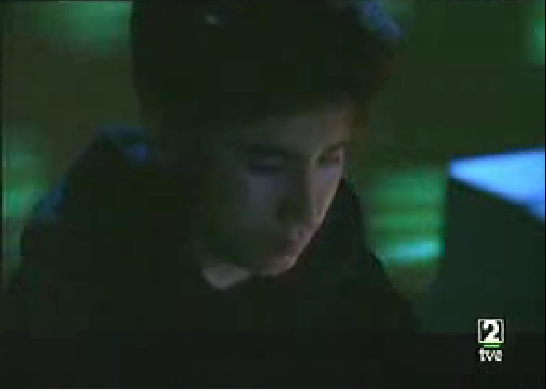
\includegraphics[scale=0.45]{imgs/documental.png}
%    %\caption{}
%  \end{figure}
%  \begin{center}
%    http://video.google.com/
%    videoplay?docid=6729008725344610785\&pr=goog-sl
%  \end{center}
%\end{frame}
%
%\begin{frame}
%  \frametitle{Actividad: Discusión de los elementos ciberculturales del video}
%  \begin{center}
%    Se deberá discutir el video anterior a la luz de los elementos aprendidos en clase.
%    \begin{itemize}
%    \item ¿Por qué creen que surgió el movimiento hacker a nivel mundial?
%    \item ¿Tiene el software libre futuro?
%    \item ¿Qué ventajas y desventajas tiene el S.L. sobre el Software Comercial?
%    \end{itemize}
%  \end{center}
%\end{frame}
%
%\begin{frame}%[allowframebreaks]
%  \frametitle<presentation>{Lecturas Recomendadas}
%
%  \begin{thebibliography}{10}
%
%    \beamertemplatebookbibitems
%  \bibitem{Pekka1996}
%    Pekka Himanen
%    \newblock {\em La ética del hacker y el espíritu de la era de la información}
%    \newblock Ediciones Destino.
%
%  \bibitem{TuxEvang}
%    Lennier <culln@xtra.co.nz>
%    \newblock {\em El evangelio según Tux}.
%    \newblock http://es.tldp.org/Humor/evangelio.txt
%
%  \bibitem{EHACK}
%    James S. Tiller.
%    \newblock {\em The Ethical Hack}.
%    \newblock A framework for business value penetration testing
%  \end{thebibliography}
%\end{frame}
%
%\begin{frame}%[allowframebreaks]
%  \frametitle<presentation>{Lecturas Recomendadas}
%
%  \begin{thebibliography}{10}
%
%    \beamertemplatebookbibitems
%  \bibitem{Velo1996}
%    Mark Dery.
%    \newblock {\em Velocidad de Escape}
%    \newblock Mark Dery.
%
%  \bibitem{Jargon}
%    Eric Raymond.
%    \newblock {\em The Jargon File}.
%    \newblock http://catb.org/jargon/
%
%  \bibitem{Howto}
%    Eric Raymond.
%    \newblock {\em How To Become a Hacker}.
%    \newblock http://www.catb.org/~esr/faqs/hacker-howto.html
%  \end{thebibliography}
%\end{frame}
%
%\section{Instalación (Duración: 5 horas)}
%\begin{frame}
%  \frametitle{Distribuciones}
%  \begin{columns}
%    \begin{column}[ht]{5cm}
%      \begin{figure}[ht]
%        \centering
%        
\includegraphics[scale=0.5]{imgs/slackware.png}
%        %\caption{}
%      \end{figure}
%      \begin{figure}[ht]
%        \centering
%        \includegraphics[scale=0.25]{imgs/fedora.png}
%        %\caption{}
%      \end{figure}
%    \end{column}
%    \begin{column}[ht]{5cm}
%      \begin{figure}[ht]
%        \centering
%        \includegraphics[scale=0.25]{imgs/debian.png}
%        %\caption{}
%      \end{figure}
%      \begin{figure}[ht]
%        \centering
%        
\includegraphics[scale=0.4]{imgs/ubuntu.png}
%        %\caption{}
%      \end{figure}
%    \end{column}
%  \end{columns}
%\end{frame}
%
%\begin{frame}
%  \frametitle{UBUNTU}
%  \begin{columns}
%    \begin{column}[ht]{5cm}
%      \begin{itemize}
%      \item Significa: ``Humanidad hacia otros''.
%      \item Orientado a PC y usuario final.
%      \item Basado en Debian.
%      \item Patrocinador: Canonical Ltda.
%      \item Versión Actual: 9.04
%      \end{itemize}
%    \end{column}
%    \begin{column}[ht]{5cm}
%      \begin{figure}[ht]
%        \centering
%        
\includegraphics[scale=0.3]{imgs/ubuntu.png}
%        %\caption{}
%      \end{figure}
%      \begin{figure}[ht]
%        \centering
%        \includegraphics[scale=0.45]{imgs/kubuntu.png}
%        %\caption{}
%      \end{figure}
%      \begin{figure}[ht]
%        \centering
%        \includegraphics[scale=0.25]{imgs/edubuntu.png}
%        %\caption{}
%      \end{figure}
%      \begin{figure}[ht]
%        \centering
%        
\includegraphics[scale=0.15]{imgs/xubuntu.png}
%        %\caption{}
%      \end{figure}
%    \end{column}
%  \end{columns}
%\end{frame}
%
%\begin{frame}
%  \frametitle{La Tabla de Particiones}
%  \begin{columns}
%    \begin{column}[ht]{5cm}
%      \begin{itemize}
%      \item Se ubica en el MBR de la máquina.
%      \item Ocupa 64 bytes. 4 Registros de 16 bytes.
%      \item Definen las particiones primarias.
%      \item Ahí se guarda toda la información básica de las particiones.
%      \end{itemize}
%    \end{column}
%    \begin{column}[ht]{5cm}
%      \begin{figure}[ht]
%        \centering
%        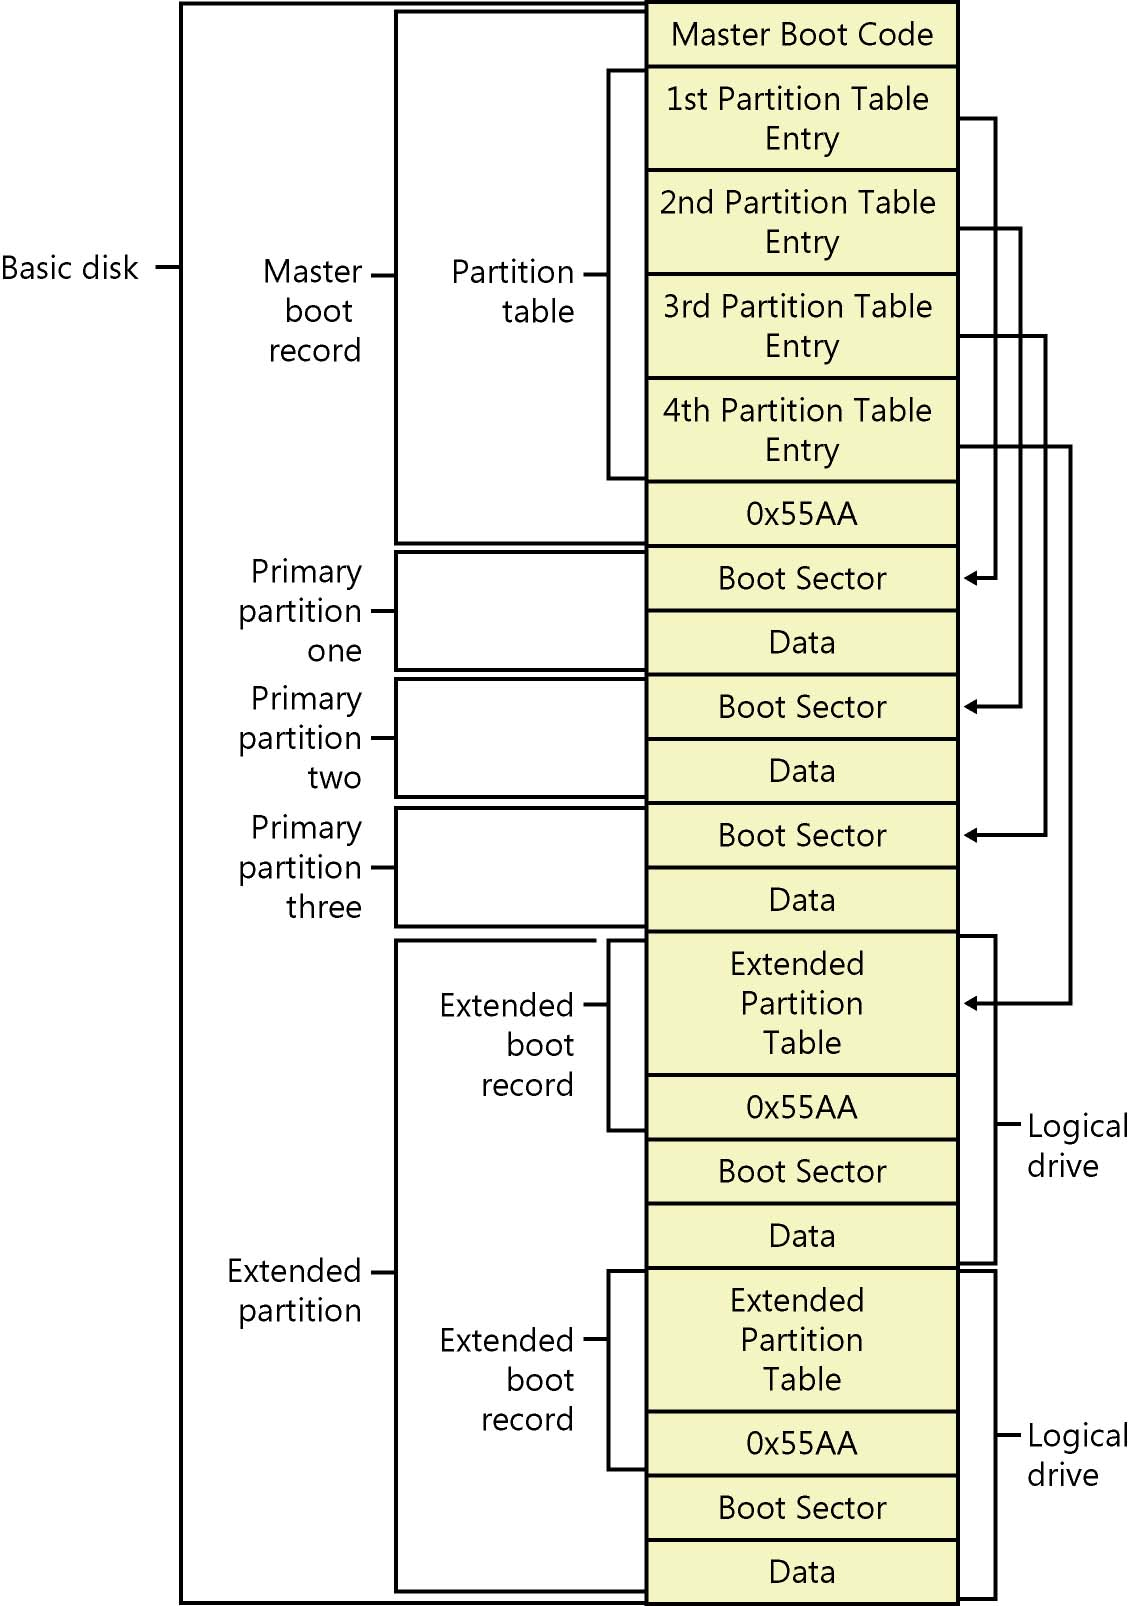
\includegraphics[scale=0.5]{imgs/tablapart.jpg}
%        %\caption{}
%      \end{figure}
%    \end{column}
%  \end{columns}
%\end{frame}
%
%\begin{frame}
%  \frametitle{Gparted}
%  \begin{itemize}
%  \item Linux Live-On CD
%  \item Manipula tabla de particiones
%  \item Permite realizar particionamiento \textit{no destructivo}
%  \item Soporta distintos sistemas de archivos
%    \begin{itemize}
%    \item NTFS
%    \item FAT
%    \item EXT3
%    \item Muchas otras!
%    \end{itemize}
%  \item También es utilizado para recuperación de información ante desastres.
%  \end{itemize}
%\end{frame}
%
%\begin{frame}
%  \frametitle{Gparted}
%  \begin{figure}[ht]
%    \centering
%    \includegraphics[scale=0.3]{imgs/gparted1.jpg}
%    \caption{Screenshot tomado de gparted.sourceforge.net}
%  \end{figure}
%\end{frame}
%
%\begin{frame}
%  \frametitle{Gparted}
%  \begin{figure}[ht]
%    \centering
%    \includegraphics[scale=0.25]{imgs/gparted2.jpg}
%    \caption{Screenshot tomado de gparted.sourceforge.net}
%  \end{figure}
%\end{frame}
%
%\begin{frame}
%  \frametitle{Gparted}
%  \begin{figure}[ht]
%    \centering
%    \includegraphics[scale=0.25]{imgs/gparted3.jpg}
%    \caption{Screenshot tomado de gparted.sourceforge.net}
%  \end{figure}
%\end{frame}
%
%\begin{frame}
%  \frametitle{Gparted}
%  \begin{figure}[ht]
%    \centering
%    \includegraphics[scale=0.35]{imgs/gparted4.jpg}
%    \caption{Screenshot tomado de gparted.sourceforge.net}
%  \end{figure}
%\end{frame}
%
%\begin{frame}
%  \frametitle{Gparted}
%  \begin{figure}[ht]
%    \centering
%    \includegraphics[scale=0.4]{imgs/gparted5.jpg}
%    \caption{Screenshot tomado de gparted.sourceforge.net}
%  \end{figure}
%\end{frame}
%
%\begin{frame}
%  \frametitle{Gparted}
%  \begin{figure}[ht]
%    \centering
%    \includegraphics[scale=0.35]{imgs/gparted6.jpg}
%    \caption{Screenshot tomado de gparted.sourceforge.net}
%  \end{figure}
%\end{frame}
%
%\begin{frame}
%  \frametitle{Gparted}
%  \begin{figure}[ht]
%    \centering
%    \includegraphics[scale=0.25]{imgs/gparted7.jpg}
%    \caption{Screenshot tomado de gparted.sourceforge.net}
%  \end{figure}
%\end{frame}
%
%\begin{frame}
%  \frametitle{Gparted}
%  \begin{figure}[ht]
%    \centering
%    \includegraphics[scale=0.45]{imgs/gparted8.jpg}
%    \caption{Screenshot tomado de gparted.sourceforge.net}
%  \end{figure}
%\end{frame}
%
%\begin{frame}
%  \frametitle{Gparted}
%  \begin{figure}[ht]
%    \centering
%    \includegraphics[scale=0.35]{imgs/gparted9.jpg}
%    \caption{Screenshot tomado de gparted.sourceforge.net}
%  \end{figure}
%\end{frame}
%
%\begin{frame}
%  \frametitle{Gparted}
%  \begin{figure}[ht]
%    \centering
%    \includegraphics[scale=0.35]{imgs/gparted10.jpg}
%    \caption{Screenshot tomado de gparted.sourceforge.net}
%  \end{figure}
%\end{frame}
%
%\begin{frame}
%  \frametitle{Gparted}
%  \begin{figure}[ht]
%    \centering
%    \includegraphics[scale=0.35]{imgs/gparted11.jpg}
%    \caption{Screenshot tomado de gparted.sourceforge.net}
%  \end{figure}
%\end{frame}
%
%
%\begin{frame}
%  \frametitle{Sistemas de Archivos}
%  \begin{itemize}
%  \item Estructura la información guardada en un dispositivo de almacenamiento, como un \textit{dvd}, \textit{hd}, \textit{pendrive}, etc.
%  \item Rutas y nombres de archivos
%  \item Seguridad
%    \begin{itemize}
%    \item ACL's
%    \item UGO
%    \item Atributos extendidos 
%    \end{itemize}
%  \item Mecanismos anti--fragmentación
%  \item Integridad del sistema de archivos
%  \item Cuotas de disco
%  \end{itemize}
%\end{frame}
%
%\begin{frame}
%  \frametitle{Requisitos Mínimos: Arquictecturas HW}
%  \begin{itemize}
%  \item Intel x86-based i386
%  \item AMD64 \& Intel EM64T amd64
%  \item HP PA-RISC hppa PA-RISC 1.1 32
%  \item PA-RISC 2.0 64
%  \item Intel IA-64 ia64    
%  \item IBM/Motorola PowerPC powerpc PowerMac pmac
%  \item Sun SPARC sparc sun4u sparc64
%  \end{itemize}
%\end{frame}
%
%\begin{frame}
%  \frametitle{Requisitos Mínimos: Medios de Instalación}
%  \begin{itemize}
%  \item CD--ROM
%  \item DVD--ROM
%  \item USB Memory Stick
%  \item Network -- NFS -- HTTP -- FTP
%  \end{itemize}
%\end{frame}
%
%\begin{frame}
%  \frametitle{Requisitos Mínimos: Memoria y Disco}
%  \begin{columns}
%    \begin{column}[ht]{5cm}
%      \begin{itemize}
%      \item 44 megas de RAM mínimo
%      \item 500 megas de disco duro mínimo
%      \item 380 megas de disco duro ideal
%      \item 4 Gigas de disco duro ideal
%      \end{itemize}
%    \end{column}
%    \begin{column}[ht]{5cm}
%      \begin{figure}[ht]
%        \centering
%        \includegraphics[scale=0.25]{imgs/ram.jpg}
%        %\caption{}
%      \end{figure}
%      \begin{figure}[ht]
%        \centering
%        \includegraphics[scale=0.25]{imgs/dd.jpg}
%        %\caption{}
%      \end{figure}
%    \end{column}
%  \end{columns}
%\end{frame}
%
%\begin{frame}[shrink=10]
%  \frametitle{Proceso de Instalación}
%  \begin{enumerate}
%  \item Hacer copia de seguridad de cualquier dato o documento importante en el disco duro donde usted planea instalar kubuntu.
%  \item Obtener información acerca de su computador y cualquier documentación que sea necesaria antes de empezar con la instalación.
%  \item Crear espacio particionable para kubuntu en su disco duro.
%  \item Localizar y/o bajar el software instalador y cualquier \textit{driver} especializado que su máquina pueda necesitar.
%  \item Configurar la manera en que se \textit{bootea} el sistema.
%  \item \textit{Bootear} el sistema de instalación.
%  \item Seleccionar el lenguaje de instalación.
%  \item Activar conexión \textit{ethernet} si está disponible (Inseguro).
%  \item Crear y montar las particiones donde Kubuntu será instalado.
%  \item Instalar y configurar el sistema base.
%  \item Instalar el cargador del boot el cual puede iniciar el Kubuntu existente. 
%  \item Correr su nuevo sistema instalado por primera vez.
%  \end{enumerate}
%\end{frame}
%
%\begin{frame}
%  \frametitle{Información Importante que debe Tener a mano}
%  \centering{Puede encontrar ésta información en:}
%  \begin{itemize}
%  \item Los manuales que vienen con cada pieza de \textit{hardware}
%  \item La BIOS del sistema
%  \item Las bolsas y las cajas del \textit{hardware}
%  \item Panel de Control de Windows
%  \item Algunos comandos del sistema
%  \item Su proveedor de Internet
%  \end{itemize}
%\end{frame}
%
%\begin{frame}
%  \frametitle{Información Importante que debe Tener a mano}
%  \centering{\alert{\textbf{Discos Duros}}}
%  \begin{itemize}
%  \item Cuántos tiene
%  \item El orden de éstos en el sistema
%  \item Si es IDE (Conocido también como PATA), SATA o SCSI.
%  \item Espacio Libre
%  \item Particiones
%  \item Particiones donde otro sistema operativo está instalado.
%  \end{itemize}
%\end{frame}
%
%\begin{frame}
%  \frametitle{Información Importante que debe Tener a mano}
%  \centering{\alert{\textbf{Monitor}}}
%  \begin{itemize}
%  \item Modelo y fabricante
%  \item Resoluciones soportadas
%  \item Tasa de refresco horizontal
%  \item Tasa de refresco vertical
%  \item Profundidad de color soportada
%  \item Tamaño de la pantalla
%  \end{itemize}
%\end{frame}
%
%\begin{frame}
%  \frametitle{Información Importante que debe Tener a mano}
%  \centering{\alert{\textbf{Mouse}}}
%  \begin{itemize}
%  \item Tipo (serial/PS2/USB)
%  \item Puerto
%  \item Fabricante
%  \item Número de botones
%  \end{itemize}
%\end{frame}
%
%\begin{frame}
%  \frametitle{Información Importante que debe Tener a mano}
%  \centering{\alert{\textbf{Red}}}
%  \begin{itemize}
%  \item Número de interfaces de red
%  \item Tipos de interfaces de red \small{(Ethernet, Wi--Fi)}
%  \item Modelo y fabricante
%  \item ¿Es soportada por Linux?
%  \item Parámetros de red de su máquina:
%    \begin{itemize}
%    \item Dirección IP
%    \item Máscara de Subred
%    \item Servidor de Nombres (DNS)
%    \item Gateway
%    \item Dominio
%    \item Grupo de Trabajo
%    \item ESSID (Si aplica)
%    \item Password (Si aplica)
%    \end{itemize}
%  \end{itemize}
%\end{frame}
%
%\begin{frame}
%  \frametitle{Información Importante que debe Tener a mano}
%  \centering{\alert{\textbf{Impresora}}}
%  \begin{itemize}
%  \item Modelo y fabricante
%  \item Resoluciones de impresión soportadas
%  \end{itemize}
%\end{frame}
%
%\begin{frame}
%  \frametitle{Información Importante que debe Tener a mano}
%  \centering{\alert{\textbf{Tarjeta de Video}}}
%  \begin{itemize}
%  \item Modelo y fabricante
%  \item Memoria RAM de video disponible
%  \item Resolución y profundidad de color soportada.
%  \end{itemize}
%\end{frame}
%
%\begin{frame}
%%  \frametitle{Instalación Kubuntu}
%\centering{\Huge{\textbf{Vamos a Instalar!!!}}}
%\end{frame}
%
%
%
%
%%% \subsection{Particionamiento}
%%% \subsection{Herramientas de particionamiento}
%%% \subsection{Particionamiento no destructivo}
%%% \subsection{Sistemas de Archivos}
%%% \subsection{Seleccion de paquetes}
%%% \subsection{Instalación del cargador de Linux (Sistema Dual)}
%%% \subsection{Configuración Inicial}
%%% \subsection{Instalación de paquetes básicos}
%%% % Dia Numero 2
%%% \section{El sistema de archivos (Duración: 1 hora)}
%%%     \subsection{Tipos de sistemas de archivos, ventajas y desventajas.}
%%%     \subsection{El árbol de directorios}
%%% \section{La Shell (Duración: 3 horas)}
%%%   \subsection{Comandos básicos}
%%%   \subsection{Histórico de Órdenes}
%%%   \subsection{Archivos . y el .bashrc}
%%%   \subsection{Variables de Entorno}
%%%   \subsection{Sustitución de ordenes y alias}
%%%   \subsection{Manipulación de Archivos y Directorios}
%%%   \subsection{Entrada, salida y error estándar}
%%%   \subsection{Tuberías}
%%%   \subsection{Programas y procesos}
%%%   \subsection{Control de trabajos}
%%%   \subsection{Busquedas, los comandos find y locate}
%%%   \subsection{Shell scripting}
%%% \section{Administración (Duración: 4 horas)}
%%%   \subsection{La cuenta de Superusuario}
%%%   \subsection{Arranque y parada del sistema (Runlevels)}
%%%   \subsection{Administración de usuarios}
%%%   \subsection{Procesos del Sistema}
%%%   \subsection{Montaje de Unidades, particiones, pendrives}
%%%   \subsection{Instalación y actualización de paquetes}
%%%   \subsection{Sistema de Audio}
%%%   \subsection{El directorio /etc y archivos de configuración}
%%%   \subsection{Señales y el comando kill}
%%% % Dia Numero 3
%%% \section{Red (Duración: 4 horas)}
%%%   \subsection{Conectividad}
%%%     \subsubsection{Modem}
%%%     \subsubsection{Ethernet 802.3}
%%%     \subsubsection{Wi--Fi 802.11}
%%%   \subsection{Configuración básica}
%%%   \subsection{Comandos de administración y Diagnósticos}
%%%   \subsection{Servicios de red}
%%%     \subsubsection{SSH}
%%%     \subsubsection{FTP}
%%%     \subsubsection{WWW}
%%%     \subsubsection{SAMBA}
%%%     \subsubsection{Cron}
%%% \section{Entornos Gráficos (Duración: 2 horas)}
%%%   \subsection{X}
%%%   \subsection{KDE}
%%%   \subsection{Gnome}
%%%   \subsection{Compiz y otras mejoras}
%%% \section{Seguridad (Duración: 2 horas)}
%%%   \subsection{Fundamentación}
%%%   \subsection{CIA}
%%%   \subsection{Antivirus, Cortafuegos y Sistema de Detección de Intrusos}
%%%   \subsection{Políticas}
%%% % Dia Numero 4
%%% \section{Aplicaciones (Duración: 5 horas)}
%%%     \subsection{Oficina}
%%%     \subsection{Diseño}
%%%     \subsection{Editores gráficos y de consola}
%%%     \subsection{Herramientas Administrativas}
%%%     \subsection{Herramientas Educativas}
%%%     \subsection{Herramientas de Programación}
%%%     \subsection{Herramientas de Compatibilidad y Virtualización}
%%% \section{Aplicaciones de Windows que existe equivalente en Linux (Duración: 1 hora)}
%%% \section{Ventajas y Desventajas de Linux comparado con otros S.O. (Duración: 1 hora)}
%%% \section{Páginas, Documentación, Recursos recomendados y Finalización del Curso (Duración: 1 hora)}
%
